%\documentclass[preprint,12pt,authoryear, review]{elsarticle}
%
%\usepackage{natbib}
%\usepackage{amssymb}
%\bibliographystyle{elsarticle-harv}
%\usepackage{multirow}
%\usepackage{multicol,caption}
%\newenvironment{Figure}
%{\par\medskip\noindent\minipage{\linewidth}}
%{\endminipage\par\medskip}
%\usepackage{array}
%\newcolumntype{L}[1]{>{\raggedright\let\newline\\\arraybackslash\hspace{0pt}}m{#1}}
%\newcolumntype{C}[1]{>{\centering\let\newline\\\arraybackslash\hspace{0pt}}m{#1}}
%\newcolumntype{R}[1]{>{\raggedleft\let\newline\\\arraybackslash\hspace{0pt}}m{#1}}
%\usepackage{indentfirst}
%\usepackage{graphicx}
%\usepackage{subcaption} 
%\usepackage[export]{adjustbox}
%\usepackage{lscape} %to insert horizontal pages
%\usepackage{rotating} %to rotate elements (like tables)
%\usepackage{siunitx}
%\sisetup{round-mode=places, round-precision=2} %
%\usepackage[most]{tcolorbox} % Text boxes
%\usepackage[left=3cm,top=2.5cm,right=2cm,bottom=2.5cm]{geometry}
%\usepackage{textcomp}
%\usepackage{gensymb} %for using \mathbf{}
%\usepackage{amsbsy} % for boldsymbol{}
%\usepackage{booktabs} 
%\usepackage{lineno}
%\usepackage{tabularx} 
%\renewcommand*\footnoterule{} 
%\usepackage{reledmac}
%\usepackage{setspace}
%\usepackage{etoolbox}
%\arrangementX[A]{twocol}
%\colalignX{\justifying}
%\makeatletter
%\bhooknoteX[A]{\setstretch {\setspace@singlespace}}
%\bhookgroupX[A]{\setstretch {\setspace@singlespace}}
%\makeatother
%\let\footnote\footnoteA
%\makeatletter
%\newcommand\footnoteref[1]{\protected@xdef\@thefnmark{\ref{#1}}\@footnotemark}
%\makeatother
\def\Plus{\texttt{+}} % for personalized plus symbol
%
%\usepackage{hyperref}
%\hypersetup{colorlinks=true} 
%\urlstyle{same}
%\journal{Journal}

%\begin{document}
%
%\begin{frontmatter}

\chapter{Climate change mitigation through irrigation strategies during rice growing season is off-set in fallow season}
\label{Chapter2}

\begin{center}
\textbf{
Sebastián Echeverría-Progulakis\textsuperscript{1},
Néstor Pérez-Méndez\textsuperscript{1},
Marc Viñas\textsuperscript{2}
Mar Carreras-Sempere\textsuperscript{2}
Miriam Guivernau\textsuperscript{2}
Lluís Jornet\textsuperscript{1}
Mar Catala-Forner\textsuperscript{3}
Maite Martínez-Eixarch\textsuperscript{1}
}
\end{center}

\vspace{1ex}

\begin{center}
\textsuperscript{1} IRTA, Marine and Continental Waters Program, La Ràpita, 43540, Catalonia, Spain \\
\textsuperscript{2} IRTA, Sustainability in Biosystems Program, Caldes de Montbui, 08140, Catalonia, Spain\\
\textsuperscript{3} IRTA, Sustainable Field Crops Program, Amposta, 43870, Catalonia, Spain  \\

\end{center}


%
%
%\author[inst1,inst2, ]{Sebastián Echeverría-Progulakis}
%
%\affiliation[inst1]{organization={Marine and Continental Waters Program, IRTA},%Department and Organization
%            city={La Ràpita},
%            postcode={43540}, 
%            state={Catalonia},
%            country={Spain}}
%
%\author[inst2,b]{Néstor Pérez-Méndez}
%\author[inst3,b]{Marc Viñas}
%\author[inst3,b]{Mar Carreras-Sempere}
%\author[inst3,b]{Miriam Guivernau}
%\author[inst1,b]{Lluís Jornet}
%\author[inst2,b]{Mar Català-Forner}
%\author[inst1, ]{Maite Martínez-Eixarch}
%
%\affiliation[inst2]{organization={Sustainable Field Crops Program, IRTA},%Department and Organization 
%            city={Amposta},
%            postcode={43870}, 
%            state={Catalonia},
%            country={Spain}}
%
%\affiliation[inst3]{organization={Sustainability in Biosystems Program, IRTA},%Department and Organization 
%            city={Caldes de Montbui},
%            postcode={08140}, 
%            state={Catalonia},
%            country={Spain}}
%
%\affiliation[ ]{organization=Corresponding authors: sebastian.echeverria@irta.cat and maite.martinezeixarch@irta.cat}
%
%\affiliation[b]{organization=Contributing authors: nestor.perez@irta.cat, marc.vinas@irta.cat, mar.carreras@irta.cat, miriam.guivernau@irta.cat, lluis.jornet@irta.cat and mar.catala@irta.cat}    
     
%\doublespacing
%\begin{abstract}
\section*{Abstract}
Non-continuous flooding irrigation practices, such as alternate wetting and drying (AWD) and mid-season drainage (MSD), have been implemented in rice agroecosystems to reduce water use and mitigate climate change. Draining fields reduces methane (CH$_{4}$) emissions, as soil aeration decreases the abundance and activity of soil methanogens. Mitigation effects during the growing season have been widely studied. However, there is a knowledge gap regarding potential effects these growing season practices might have on subsequent fallow season emissions. This is relevant when assessing overall annual CH$_{4}$ emissions, particularly in systems in which fallow seasons account for a significant part of these. A field experiment was implemented in the Ebro Delta region (Catalonia, Spain) with the objective of identifying potential effects of growing season AWD and MSD on CH$_{4}$ emitted during the following flooded fallow season, in comparison to continuously flooded fields. Changes in the structure of soil microbial communities were also characterized. Both emissions and microbial communities were analyzed for rice field plots under the assessed irrigation strategies during the growing season and later for a continuously flooded mesocosm across the fallow season. Both practices achieved an average 86\% decrease in CH$_{4}$ fluxes when compared to continuous flooding during the growing season. AWD resulted in the highest fallow season emissions, leading to increases in overall annual cumulative CH$_{4}$ emissions (\Plus 8\%), global warming potential (\Plus 30\%) and yield-scaled global warming potential (\Plus 70\%) compared to continuous flooding. Growing season AWD decreased the relative abundance of both methanogens and methanotrophs in the fallow season. Reduced methanotroph communities might lead to lower CH$_{4}$ consumption, resulting in higher fallow season emissions and offsetting the mitigation effect achieved during the growing season. Under the studied conditions, MSD represented a more effective mitigation strategy. These results highlight the importance of considering both rice growing and fallow season when assessing climate change mitigation strategies.\\ 

%\end{abstract}

%\begin{keyword}
%% keywords here, in the form: keyword \sep keyword
\noindent\textbf{Keywords:}Greenhouse gas emissions; paddy rice; water management; legacy effects; soil microbiology 

%\end{keyword}

%\end{frontmatter}

%\linenumbers

%\doublespacing

\section{Introduction}
\label{sec:intro}

% PAR 1: Rice and its importance in food security and GHG emissions

Rice (\textit{Oryza sativa L.}) is a major staple crop and the third largest harvested area worldwide, accounting for approximately 11\% of total arable land \citep{Faostat2022}. Besides its critical role as food source, paddy rice cultivation is also a key anthropogenic driver of greenhouse gas (GHG) emissions \citep{bouman2007rice, nabuurs2022agriculture}. Most rice systems are managed under continuous flooding during a major part of the growing season, leading to high methane (CH$_{4}$) emissions due to favored anaerobic metabolic pathways within soil microbial communities \citep{conrad2007microbial, perry2024}. When paddy fields are drained, higher oxygen availability in soils promotes nitrous oxide (N$_{2}$O) production and emission \citep{cai1997methane}. Both CH$_{4}$ and N$_{2}$O are among the three most important GHG in the atmosphere, after CO$_{2}$, and contribute 27 and 273 times more, respectively, to global warming potential (GWP) than CO$_{2}$ at a 100 year time horizon \citep{IPCC2021}. Overall, rice production accounts for 11\% of total anthropogenic emissions of these non-CO$_{2}$ emissions \citep{Smith2007}.\\ 

% PAR 2: Context of flooded fallow (as suggested by Reviewer #4):

Winter flooded fallow season is a practice restricted to particular rice production areas, such as in the US (e.g. California, \cite{fitzgerald2000}; Arkansas, \cite{reba2019}), China (12\% of total cultivated area, \cite{zhang2011}), Spain and some reduced areas in southern France and northern Italy \citep{pernollet2015}. This practice has been promoted by policies aiming at enhancing waterbird habitat creation \citep{elphick2010, tajiri2013effects}, replacing straw burning practices (i.e., by increasing incorporated straw decomposition rates), and due to several other agronomic benefits (e.g. limiting erosion, inhibiting weed seed germination and retaining sediments and nutrients; \cite{negri2020}). In the Ebro Delta (Catalonia, Spain) rice production region, keeping fields flooded during winter is a common practice to improve straw decomposition but mainly to preserve its status of biodiversity hotspot \citep{day2006, perez-mendez2022}. Flooding fallow fields, nevertheless, increases both winter and subsequent growing season CH$_{4}$ emissions in comparison to drained fallow fields \citep{cai2000}. In flooded fallow rice systems, decreased rates of straw input and nitrogen fertilization  have been found to decrease fallow CH$_{4}$ emissions \citep{martinez-eixarch2021a}. Furthermore, positive effects of field drains during previous growing seasons have been identified to extent into fallow season emissions \citep{martinez-eixarch2022}, but there is still a lack of studies comparing the effect of different irrigation strategies on overall annual emissions.\\

% PAR 3: Alternative water managements to permanent flooding as effective CH4 mitigation measures

Awareness of rice contribution to climate change is driving an increase in research efforts to develop adaptation and mitigation strategies in its production \citep{alexandratos2012world, zhang2018effect, hussain2020rice}. Rice irrigation practices involving drainage conditions, such as alternate wetting and drying (AWD), consisting of several flooding-drainage cycles through the growing season, and mid-season drainage (MSD), with just one drain event in the season, have been largely studied and implemented \citep{li2004, li2014, lampayan2015}. The principle behind these strategies is that introducing aerobic conditions to soils inhibits the activity of anaerobic methanogenic archaea, thus reducing CH$_{4}$ emissions \citep{kumar2019alternate, perry2024}. Whereas these practices are effective in reducing emissions by 53\% on average during the growing season \citep{jiang2019water}, little is known about how their effects extend into subsequent flooded fallow seasons, which in temperate production areas can account up to 70\% of overall annual emissions \citep{martinez2018neglecting}. Draining events during the growing season might, for instance, drive long lasting changes in the activity and composition of microbial communities that can be extended to the fallow season, ultimately affecting overall emission outcomes. \\

% PAR 4 - after Reviewer's #4 suggestion: Legacy effects

Impacts that previous conditions might have on current processes and properties, have been termed as legacy effects, a concept that has been applied in the context of climate change to describe how ecological legacies result from feedbacks between biotic, soil, and geomorphic processes \citep{monger2015legacy}. Legacy effects of previous land and water management in rice paddy fields on soil organic matter content, structures of soil microbial communities and, therefore, CH$_{4}$ and N$_{2}$O emissions have been identified \citep{shao2017, tian2022}. Characterizing the main factors driving such effects is crucial to understanding potential outcomes of implementing mitigation practices. On one hand, constant high soil carbon inputs through straw incorporation after each year rice harvest correlates positively to incremental CH$_{4}$ emissions, up to a threshold of CH$_{4}$ production is reached \citep{hatala2012}. On the other, long term continuous flooding management increases the abundance of soil methanogens and CH$_{4}$ emissions, compared with soils under non-continuous flooding practices, due to a progressive adaptation of microbial communities to irrigation management \citep{lagomarsino2016a}.\\

% PAR 5  - after Reviewer's #4 suggestion: Our hypothesis

In this context, this study was set to determine potential legacy effects of water management practices implemented during the rice growing season on CH$_{4}$ emissions during a flooded fallow season. During the previous season (2022), AWD resulted in 12,9\% grain yield decrease versus continuously flooded plots. Similar decreases in current yields would probably mean a decrease in carbon inputs, due to less biomass produced and less straw incorporated. Additionally, MSD had previously been identified as a practice with mitigation effects lagging onto the fallow season in the studied site \citep{martinez-eixarch2022}. Such background supported the hypothesis of non-continuous flooding strategies maintaining their positive climate mitigation effect into the fallow season, through a decrease in CH$_{4}$ emissions, led by decreased carbon inputs and lower methanogen abundance than in microbial communities adapted to continuous flooding conditions. To test this hypothesis we specifically characterized the following issues across the three assessed irrigation strategies: i) CH$_{4}$ emission patterns during both growing and fallow season, ii) GWP and yield scaled global warming potential (GWPY), iii) microbial community composition during both periods, and iv) relative abundance of microbial functional groups related to CH$_{4}$ metabolism (i.e., methanogens and methanotrophs) during the flooded fallow season.\\

\section{Materials and methods}
\label{sec:meth}

\subsection{Study site}
\label{sec:meth_Site}

Experiments were set within the IRTA Ebro Experimental Station facilities in Amposta, Ebro Delta, Catalonia, Spain (40°42’88 30.2” N, 0°37’ 56.5” E). This deltaic region covers a surface of 320 km$^2$, where natural ecosystems contrast with rice paddy fields, which dominate the overall landscape \citep{romagosa2013sustainability}. Around 210 km$^2$ are managed as rice fields, accounting for 65\% of the total surface. The conventional local practice is to keep these fields under continuous flooding for most of the growing season (May to early October). During the fallow season subsequent to rice harvest (October to December), the remaining straw is chopped and incorporated before winter flooding \citep{martinez-eixarch2021a}. Flooding and draining large surfaces of paddy fields is accomplished thanks to a complex channel network transporting freshwater from the Ebro river. These irrigation practices require a constant input of large volumes of freshwater, and this high water demand is in conflict with current regional water availability. The Meteorological Service of Catalonia declared the current drought as the worst in record, being 2023 the second-driest year, only after 2022 \citep{MeteoCat2024}. 

\subsection{Experimental layout}
\label{sec:meth_Exp}

During the 2022 and 2023 rice growing and fallow seasons, a field experiment was conducted to assess the effect of water irrigation strategies implemented during growing seasons on GHG emissions during a flooded fallow season. Crop and water management was similar across both years. All samplings and results in this study correspond to the second year of this experiment (2023), representing, therefore, the cumulative effect of two growing seasons of water irrigation strategies on this second year fallow season. All growing season CH$_{4}$ emission (fluxes and cumulative), GWP, GWPY and grain yield presented results correspond as well to the second year of this experiment. The experiment consisted of 15 paddy rice plots of $10 \times 11$ m each. These were distributed in five blocks, each with three plots randomly assigned to one of three assessed irrigation strategies (experimental treatments): (i) conventional continuous flooding (CON), in which plots were kept flooded through the entire growing season; (ii) mid-season drainage (MSD), consisting on a single 11-days drain event before panicle initiation (June 22$^{nd}$ to July 3$^{rd}$); and (iii) alternate wetting and drying (AWD), strategy in which plots are flooded and drained cyclically through the growing season starting from 4-leaf stage (June 8$^{th}$) onwards (Figure \ref{treat}; Table \ref{field_mgmt}). Individual drainage channels were set up for each plot, allowing independent water management. All plots were water seeded at a rate of 500 seeds m$^{-2}$. To avoid strong yield declines, AWD plots were kept flooded in between heading and the end of flowering (July 3$^{rd}$-25$^{th}$) and managed under the Safe-AWD protocol \citep{bouman2007a}, setting 15 cm below ground level as water level threshold triggering plot re-flooding. Fertilization was carried out through the application of a granulated controlled-released fertilizer (33\% N, 9\% P, 6\% K) on a dose of 190 kg ha$^{-1}$. All plots were drained for three days (June 27$^{th}$-29$^{th}$) due to an herbicide and fungicide application and then later in the season, 20 days before harvest, to allow harvester access. All plots were seeded with JSendra, a commercial round rice variety predominant in the Ebro Delta area. Soil texture at the study site is silty clay (49.3\% clay; 43.8\% silt; 6.9\% sand). For a detailed description of soil physicochemical properties and nutrient content see Table \ref{straw} (containing soil analysis results from a sample composed of sub-samples from all 15 field plots).\\ 

\begin{figure} [ht]
\captionsetup{justification=justified}
	\centering 
	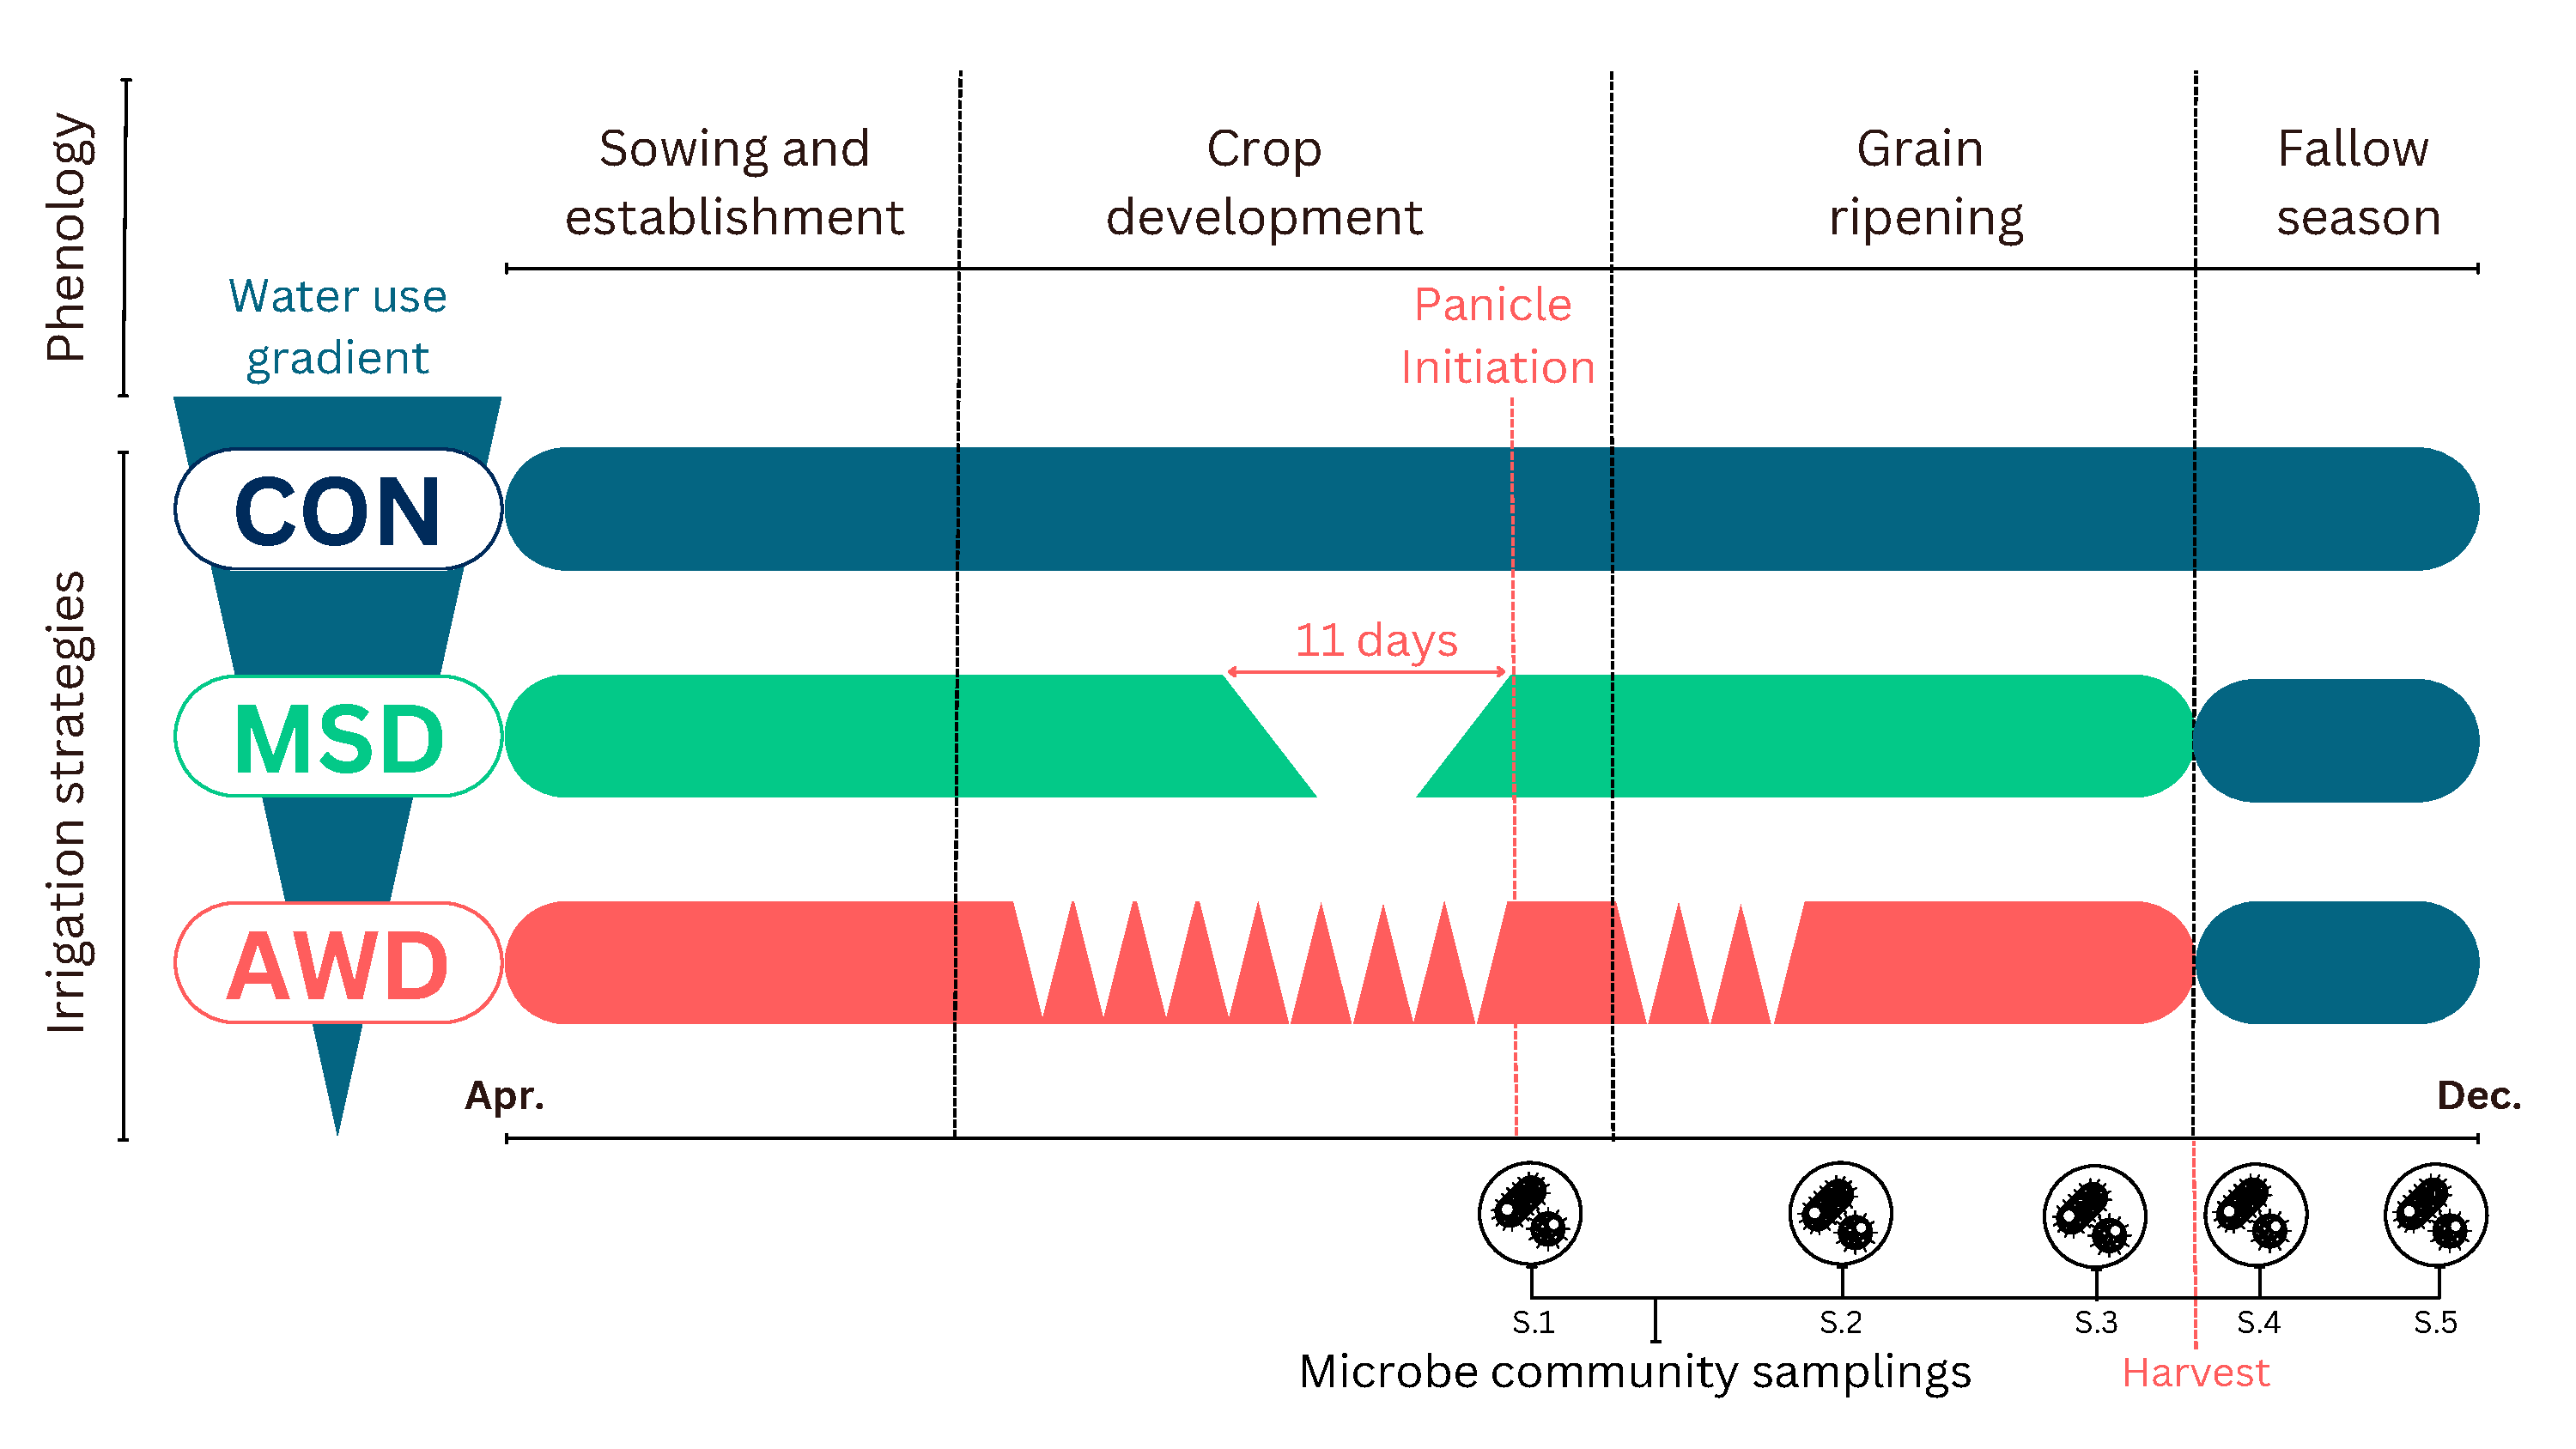
\includegraphics[scale=0.3, center]{Figures/Chapter_2/CERESTRES_Layout_2023_GSFS.pdf}
	\captionof{figure}[lay]{Assessed irrigation strategies. Horizontal bars represent the water layer for each assessed irrigation strategy across a decreasing water use gradient: conventional continuous flooding (CON); mid-season drainage (MSD); and alternate wetting and drying (AWD). Strategies are depicted for phenological stages across the growing season. The fallow season corresponds to continuous flooding for all plots. Microbe community samplings (S.1 to S.5) are shown in reference to the corresponding date and water treatment period in which they were collected: growing season (S.1, S.2 and S.3); and fallow season (S.4 and S.5).}
	\label{treat}
\end{figure}
%\vspace{0.5cm}

As an adaptation practice towards current severe droughts in the region, water available for irrigation in agriculture was halved throughout rice growing season by the local water administration. Blocking connections between main and individual plot input channels, plus keeping high water levels in individual plot drainage channels, allowed us securing continuous flooding and avoided unscheduled plot drains during main channel cuts due to this regional measure. These practices minimized potential negative effects drought might have caused on the representability of our study. Similar emission rates and trends to those registered in previous studies within the same site confirm this \citep{martinez-eixarch2021a}. A potential stop in irrigation water inflows after harvest meant risking the fallow season section of this study as field plots would have been left out of water inputs to maintain them flooded. To avoid this, the fallow season experimental layout was modified from field plots into a mesocosm experiment. The same day field plots were harvested (October 3$^{rd}$), rice plants located in a $50 \times 50$ cm frame for each plot, in which non-steady GHG sampling chambers had been installed during the growing season (see section \ref{sec:meth_GHG}), were hand harvested and grains were stored to be then added to each plot final yield. Straw residues from plants harvested within these frames were sun dried for 72 hours and chopped into 10 cm sections, emulating local open air straw drying periods and post-harvest mechanized chopping practice. After hand harvest, soil from these frames was removed down to 18 cm deep, placed within plastic boxes (54 $\times$ 48 $\times$ 37 cm, from now referred as mesocosm units), labeled according to its corresponding original field plot, and saturated with water. After three days, collected and sun dried straw was weighed to determine dry weight and incorporated by hand to each box. All irrigation strategies resulted in similar aboveground biomass, thus similar amounts of straw were incorporated to all mesocosm units (Table \ref{straw}). Soil boxes were then flooded up to 5 cm above soil level and kept flooded to this level all through the fallow season (Figure \ref{meso}). Wetland soil mesocosm experiments have proven a controlled, practical and representative methodology in previous wetland research on the fields of GHG emissions \citep{capooci2019experimental} and structure of soil microbial communities \citep{donato2020nitrogen}. Mesocosm unit representativeness of field plot soil conditions was assessed comparing physicochemical parameters with field measurements from previous flooded fallow seasons in the same experimental station (same soil texture). All assessed parameters in mesocosm units varied within similar ranges and behaved through the fallow season accordingly to previous field measurements (Figure \ref{meso_field}). \\

\begin{table*} [htbp]
    \centering
    \footnotesize  
    \begin{tabular}{ l  l  l }
\cline{1-3}
{Season} & {Date} & {Management} \\
\cline{1-3}
\rule{0pt}{3ex} % inserts space
{Growing} & {25-Apr-23} & {Fertilization (granulated controlled-release; NPK=33-9-6; 190 kg ha$^{-1}$)} \\
{} & {30-Apr-23} & {Flooding (all plots)} \\
{} & {02-May-23} & {Sowing (var. JSendra; 500 seeds m$^{-2}$)} \\
{} & {18-May-23} & {Herbicide treatment (Clincher)} \\
{} & {08-Jun-23} & {Start of first drain-flood cycle in  AWD plots} \\
{} & {22-Jun-23} & {MSD plots drained} \\
{} & {28-Jun-23} & {Herbicide treatment (Logan + Kaos)} \\
{} & {03-Jul-23} & {MSD plots re-flooded; end of first drain-flood cycles in  AWD plots} \\
{} & {25-Jul-23} & {Start of second drain-flood cycle in  AWD plots} \\
{} & {31-Jul-23} & {Fungicide treatment (Trifloxystrobin)} \\
{} & {11-Aug-23} & {End of second drain-flood cycles in  AWD plots} \\
{} & {15-Sep-23} & {Final drain (all plots)} \\
\rule{0pt}{3ex}
{Fallow} & {03-Oct-23} & {Harvest; hand harvest of frames for mesocosm setup; filling of mesocosm units} \\
{} & {06-Oct-23} & {Straw integrated to mesocosm units; flooding of mesocosm units}\\
\cline{1-3}
    \end{tabular}
    \caption{Crop treatments, experimental setup and irrigation management schedule.}
    \label{field_mgmt}
\end{table*} 

\subsection{Greenhouse gas flux measurement}
\label{sec:meth_GHG} 

For both growing and fallow seasons, GHG emissions were sampled weekly according to the non-steady chamber method, adapted from \cite{martinez2018neglecting}. Due to time and logistic constraints regarding the need of simultaneous sampling for data comparability, GHG emission samples were collected from three of the five experimental blocks throughout both growing and fallow seasons. Sample collection was done always on the same three blocks. 
% removed after Reviewer #4's suggestions: For each sample date, four 30 ml gas samples were taken every 10 minutes over a 30 minutes sampling period from each chamber using syringes. Sampled air was then transported into pre-evacuated 12.5 ml glass vials (Labco Ltd., Buckinghamsire, UK). Samplings were made in between 09:00 and 14:00 to minimize variability from daily GHG emission curves. Gas samples were then analysed in laboratory to determine GHG concentrations using a THERMO TRACE 2000 (Thermo Fisher Scientific, USA) gas chromatograph equipped with a flame ionization detector (FID, Trace GC 2000, Thermo Finnigan, Germany). 
For each sampling date, soil (electrical conductivity, temperature, redox potential and pH; all measured at 10 cm-depth) and water (temperature, salinity, oxygen concentration, oxygen saturation and pH) physicochemical parameters were registered. These parameters were assessed using an automated YSI Professional Plus (Pro Plus) Multiparameter Instrument (Brannum Lane, USA), a Hanna Instruments HI 98190 pH/ORP pH-meter and a Fieldscout direct soil E.C. meter (Spectrum Technologies, 2019). Additionally, GWP and GWPY were calculated for each irrigation strategy and rice season according to the \cite{IPCC2021} guidelines. Yield was recorded from final field plots harvest in Mg ha$^{-1}$ at 14\% humidity.\\

\subsection{Microbial biodiversity assessment}
\label{sec:meth_BIO}

Soil cores were collected from all field plots and mesocosm units to characterize microbial communities and their dynamics. A total of five soil sampling events were conducted, three during  the growing season and two during the fallow season. Growing season samplings were done after MSD drainage and first period of AWD cycles (Figure \ref{treat}, microbe community sampling S.1, July 5$^{th}$); after the second period of AWD cycles (S.2, August 16$^{th}$); and before harvest (S.3, September 5$^{th}$). During the fallow season, samplings were carried out a week after harvest, three days after straw incorporation (S.4, October 11$^{th}$); and during mid fallow season, 31 days after straw incorporation (S.5, November 6$^{th}$). \\
% removed after Reviewer #4's suggestions: During the growing season samplings, three cores were collected from each field plot, whereas only one core was collected per mesocosm unit during the two fallow season samplings. From all collected cores across seasons, top (0 to 3 cm) and bottom (5 to 10 cm) sub-samples were collected. The three top sub-samples collected per plot during the growing season were merged together, the same procedure was repeated for bottom sub-samples, obtaining one top and one bottom merged sub-sample per plot. These sub-samples were collected in 1.5 mL sterile tubes and transported to the lab at -4 \degree C, where they were frozen at -20 \degree C.\\

Total DNA was extracted from 250 mg of soil sub-samples using DNeasy\textsuperscript{\textregistered}
PowerSoil\textsuperscript{\textregistered} (Qiagen), according to manufacter's instructions. Quantitative analysis of total microbial population was conducted in the V3 hypervariable region for total bacterial population (16SrRNA F341/R518) and methanogenic archaea (mcrA gene ME1F\_qPCR y ME3R\_qPCR), as described by \cite{sotres2015}. All qPCR reactions were conducted in an AriaMx System (Agilent, USA)  and all samples were analyzed in triplicate by means of three independent cDNA/DNA extracts. Bacteria and archaea population diversity, structure and taxonomy assignment were developed according to \cite{carreras-sempere2024}.\\

% removed after Reviewer #4's suggestions: Bacteria and archaea population diversity, structure and taxonomy assignment were developed using Next Generation Sequencing technology. PCR products were sequenced through the Illumina Novaseq sequencer by an external laboratory under the 16S Metagenomic Sequencing Library Preparation protocol.

\subsection{Data analysis}
\label{sec:meth_Stat}

% Models for GHG fluxes:
For each GHG sampling event, gas-chromatography concentration results were first converted into gas areal density according to the Ideal Gas Law: 

\begin{equation} \label{GHG_a}
GHG_{a} = (\frac{M_w \times [GHG_{ppm}] \times h_m  \times 10^3}{r  \times t^{\circ}})
\end{equation}\\

where GHG$_{a}$ is the GHG areal density (in mg m$^{-2}$), M$_{w}$ is the gas molecular weight (e.g. M$_{w}$ = 12 for C-CH$_{4}$), [GHG$_{ppm}$] is the gas concentration (in ppm), h$_{m}$ is the height of the chambers (in m), in \textit{r} is the ideal gas constant (82.0575 cm$^{2}$ atm mol$^{-1}$ K$^{-1}$) and t$^{\circ}$ is the chamber temperature (in K). These results were used afterwards to build up linear models from which the resulting slopes were calculated and considered as corresponding gas fluxes as:\\

\begin{equation}
GHG_{f} = (\frac{\Delta GHG_{a}}{\Delta time})
\end{equation}\\

where GHG$_{f}$ is the GHG flux (in mg m$^{2}$ h$^{-1}$), $\Delta$GHG$_{a}$ is the difference in GHG areal densities within the chambers throughout the sampling event, and $\Delta$time is the sampling time (in hours). To avoid inconclusive data, linear models resulting in R$^{2}$ lower than 0.7 were considered non-significant linear trends, not meeting the method's detection limit or as products of ebullition induced by chamber installation, and were considered as zero flux sample events \citep{schultz2023}. For each linear model, four alternative models were tested, each removing one of the four concentrations sampled, if the original complete model had R$^{2}$ lower than 0.7 but one or more alternative models accomplished to overcome this threshold, the alternative model with higher R$^{2}$ was considered for GHG flux calculation. Cumulative GHG emissions were calculated considering constant flux in between sampling events as:

\begin{equation}
GHG_{c} = \sum_{i=1} ^{n}(\frac{GHG_{f\space i} \times \Delta time_{i+1}}{100})
\end{equation}\\

where GHG$_{c}$ is cumulative GHG emissions (in kg ha$^{-1}$) in between the \textit{i$^{th}$} and the \textit{n$^{th}$} sampling events, $\Delta$GHG$_{f \space i}$ is the GHG flux (in mg m$^{2}$ h$^{-1}$) for the \textit{i$^{th}$} sampling event, and $\Delta$\textit{time$_{i+1}$} is the time difference (in hours) in between the \textit{i$^{th}$} and the following \textit{(i+1)$^{th}$} sampling events. Calculations and data visualization were carried out using RStudio software \citep{team2020integrated}. The effects of irrigation strategies on GHG fluxes was analyzed using a Generalized Linear Mixed Models (GLMM) approach. The R package \textit{glmmTMB} was used for this purpose \citep{bolker2019getting}. Random effects were accounted for by the inclusion of treatment blocks in the model. The interaction effect between irrigation strategies and rice season was defined within the model. To account for potential temporal variation in GHG emissions, the order of the weekly samplings was included as a factor in the model, which also included soil and water physicochemical parameters as covariates. The model was fitted using Gaussian distribution and a \textit{log} link function, after performing an assessment of regression models with the \textit{performance} R package \citep{ludecke2021performance}. Model diagnostics were run to check for R$^{2}$, in addition to potential collinearity and singularity issues in the model (R package \textit{performance}). Residual distribution was checked with R package \textit{DHARMa} \citep{dharm2020residual}, to avoid residual patterns (e.g., non-normal distribution or heteroscedasticity). Once significant differences were found, \textit{emmeans} R package \citep{lenth2019emmeans} was used to run pairwise comparisons among factors. The effect of irrigation treatments on cumulative CH$_{4}$ emissions, GWP and GWPY was carried out performing a Kruskal-Wallis test and post-hoc pairwise Wilcoxon rank sum test to identify differences among irrigation strategies \citep{wust-galley2023}.\\

% Microbe biod. stats:
Microbial diversity was determined processing raw data (fastq files) from 16S rRNA-metabarcoding assessment of bacteria and archaea through R package \textit{DADA2} \citep{callahan10high}. Data processing consisted on filtering, trimming, denoising and merging paired reads resulting from the removal of primers from the demultiplexed forward (R1) and reverse (R2) reads. Chimeric sequences were identified and removed. Taxonomic amplicon sequence variants (ASV) affiliation was assigned for total bacteria and archaea using the naïve Bayesian classifier method \citep{wang2007} and the SILVA Release 138 database training set, compiling to each taxonomic level and setting a bootstrap cut-off of 70\%. \textit{DADA2} data processing procedure was applied according to its online tutorial (\url{https://benjjneb.github.io/dada2/tutorial.html}, accessed on July 1$^{st}$, 2024). Sample rarefaction by the minimum sample reads and further abundance and diversity analyses were done using the \textit{microeco} R package \citep{liu2021microeco}. Beta diversity was characterized through permutational multivariate analyses of variance (PERMANOVA) of ASV distributions based on Bray–Curtis distances with 999 permutations. The separation pattern in microbial communities and the differences among samples were identified and visualized performing a principal coordinate analysis (PCoA) based on Bray–Curtis dissimilarity. Functional profiles of soil archaea and bacteria were assigned according to the FAPROTAX database \citep{louca2016decoupling}. 
% removed after Reviewer #4's suggestions: As no evident trends differences were identified between top and bottom sub-samples, core depth as a factor was removed from the analysis and each sub-sample was considered as a sampling repetition. 
The effects of irrigation strategies on total and relative abundance of bacteria and methanogenic archaea was analyzed through a GLMM approach accounting for the interaction effect between irrigation strategies and rice season, with sampling events included as a factor independent variable and random effects accounted for by the inclusion of treatment blocks in the model. Fitted models used negative binomial distribution for total abundances and Gaussian distribution for relative abundances, after performing an assessment of regression models with the \textit{performance} R package \citep{ludecke2021performance}. Relative abundance was log transformed for methanogens to avoid residuals to deviate significantly from the model predicted values. No transformation was necessary for the methanotroph relative abundance model. Model assessment and posterior statistical analysis was the same as that described for CH$_{4}$ fluxes.\\ 

\section{Results}
\label{sec:results}

\subsection{GHG emissions} 

%\begin{landscape}
\begin{figure} [ht]
\captionsetup{justification=justified}
	\centering 
	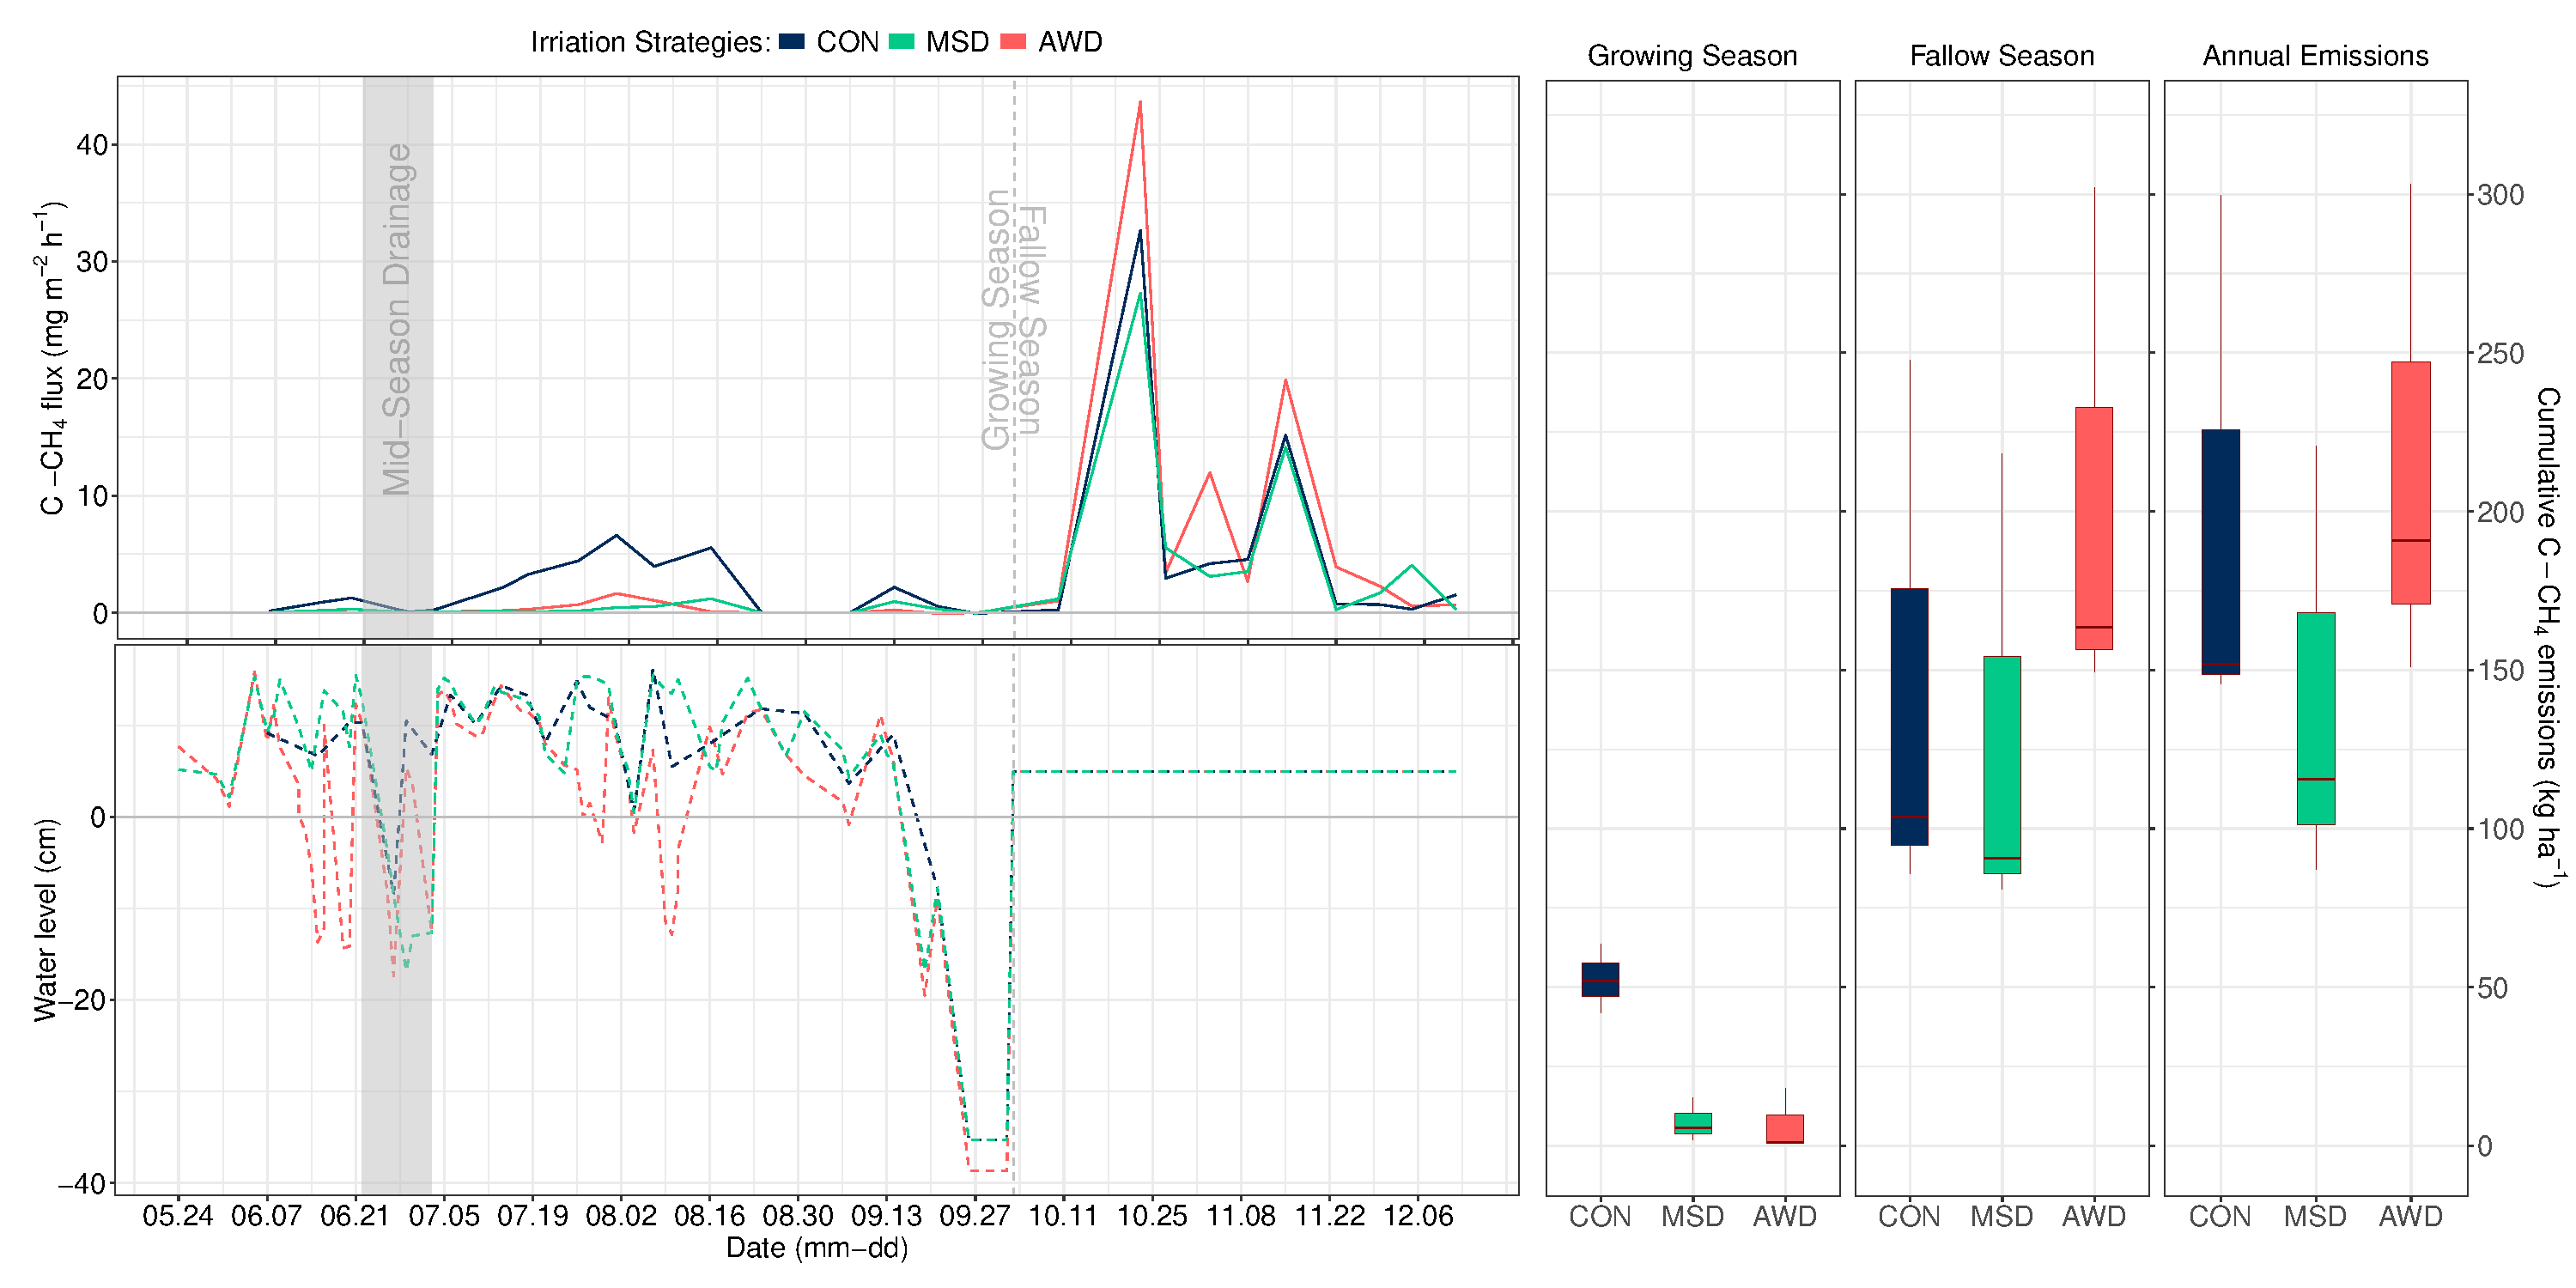
\includegraphics[scale=0.33, center]{Figures/Chapter_2/CH4_flux_water_acc.pdf}
	\captionof{figure}[CH4N2O]{Methane (CH$_{4}$, top-left panel) emission rates in mg m$^{-2}$ h$^{-1}$, and water level (bottom-left panel) in cm across the rice growing season for the three assessed irrigation strategies. Top-left panel lines are mean emissions per plot. Right boxplot panels show cumulative CH$_{4}$ emissions in kg ha$^{-1}$ for the rice growing season, fallow season and annual emissions.}  
	\label{CH4N2O}
\end{figure}
%\vspace{0.5cm}
%\end{landscape}

Fallow season emissions contributed an average of 87\% to overall annual cumulative CH$_{4}$ emissions, considering all assessed irrigation strategies, concentrated in three distinct sampled emission events rather than maintaining a constant seasonal pattern (Figures \ref{CH4N2O} and \ref{CH4_plot}). A significative interaction effect between season and irrigation treatments was identified ($\chi^2$=30.9, \textit{p}=$<$0.001). Emission patterns were inverted when transitioning from growing to fallow season. During the growing season, continuously flooded CH$_{4}$ fluxes were significantly higher than both AWD (\textit{z}=6.7, \textit{p}=$<$0.001) and MSD (\textit{z}=6.8, \textit{p}=$<$0.001) strategies. Fallow season emissions in AWD resulted higher than in continuous flooding (\textit{z}=1.9, \textit{p}=0.060) and MSD (\textit{z}=2.2, \textit{p}=0.031); no differences were registered in between continuously flooded and MSD plots (\textit{z}=0.2, \textit{p}=0.813). Model covariates such as water level ($\chi^2$=7.5, \textit{p}=0.006), soil temperature ($\chi^2$=21.3, \textit{p}=$<$0.001), atmospheric temperature ($\chi^2$=22.2, \textit{p}=$<$0.001) and soil electrical conductivity ($\chi^2$=11.3, \textit{p}=$<$0.001), as well as sampling date ($\chi^2$=12.4, \textit{p}=$<$0.001) as a model factor, resulted in significant effects on CH$_{4}$ emission rates. N$_{2}$O fluxes peaked in AWD plots during drainage periods, but also some emissions registered in plots under anoxic conditions (Figure \ref{N2O}). During the growing season, CH$_{4}$ emissions in continuously flooded plots averaged 52.5$\pm$6.2 kg ha$^{-1}$, while both non-continuous flooding strategies decreased these in approximately 86\%, with 6.8$\pm$5.7 and 7.6$\pm$3.9 kg ha$^{-1}$ emitted on average in MSD and AWD, respectively. The irrigation strategy with highest fallow season CH$_{4}$ emissions was AWD (205.1$\pm$48.7 kg ha$^{-1}$), followed by continuous flooding (145.7$\pm$51.2 kg ha$^{-1}$) and MSD (129.9$\pm$44.2 kg ha$^{-1}$). Considering overall annual cumulative CH$_{4}$ emissions, AWD (214.9$\pm$45.5 kg ha$^{-1}$) represented an 8\% increase in regards to continuously flooded (198.9$\pm$50.3 kg ha$^{-1}$) and 52\% to MSD (141.1$\pm$40.6 kg ha$^{-1}$) plots. 
\\ 

\begin{figure} [ht]
\captionsetup{justification=justified}
	\centering 
	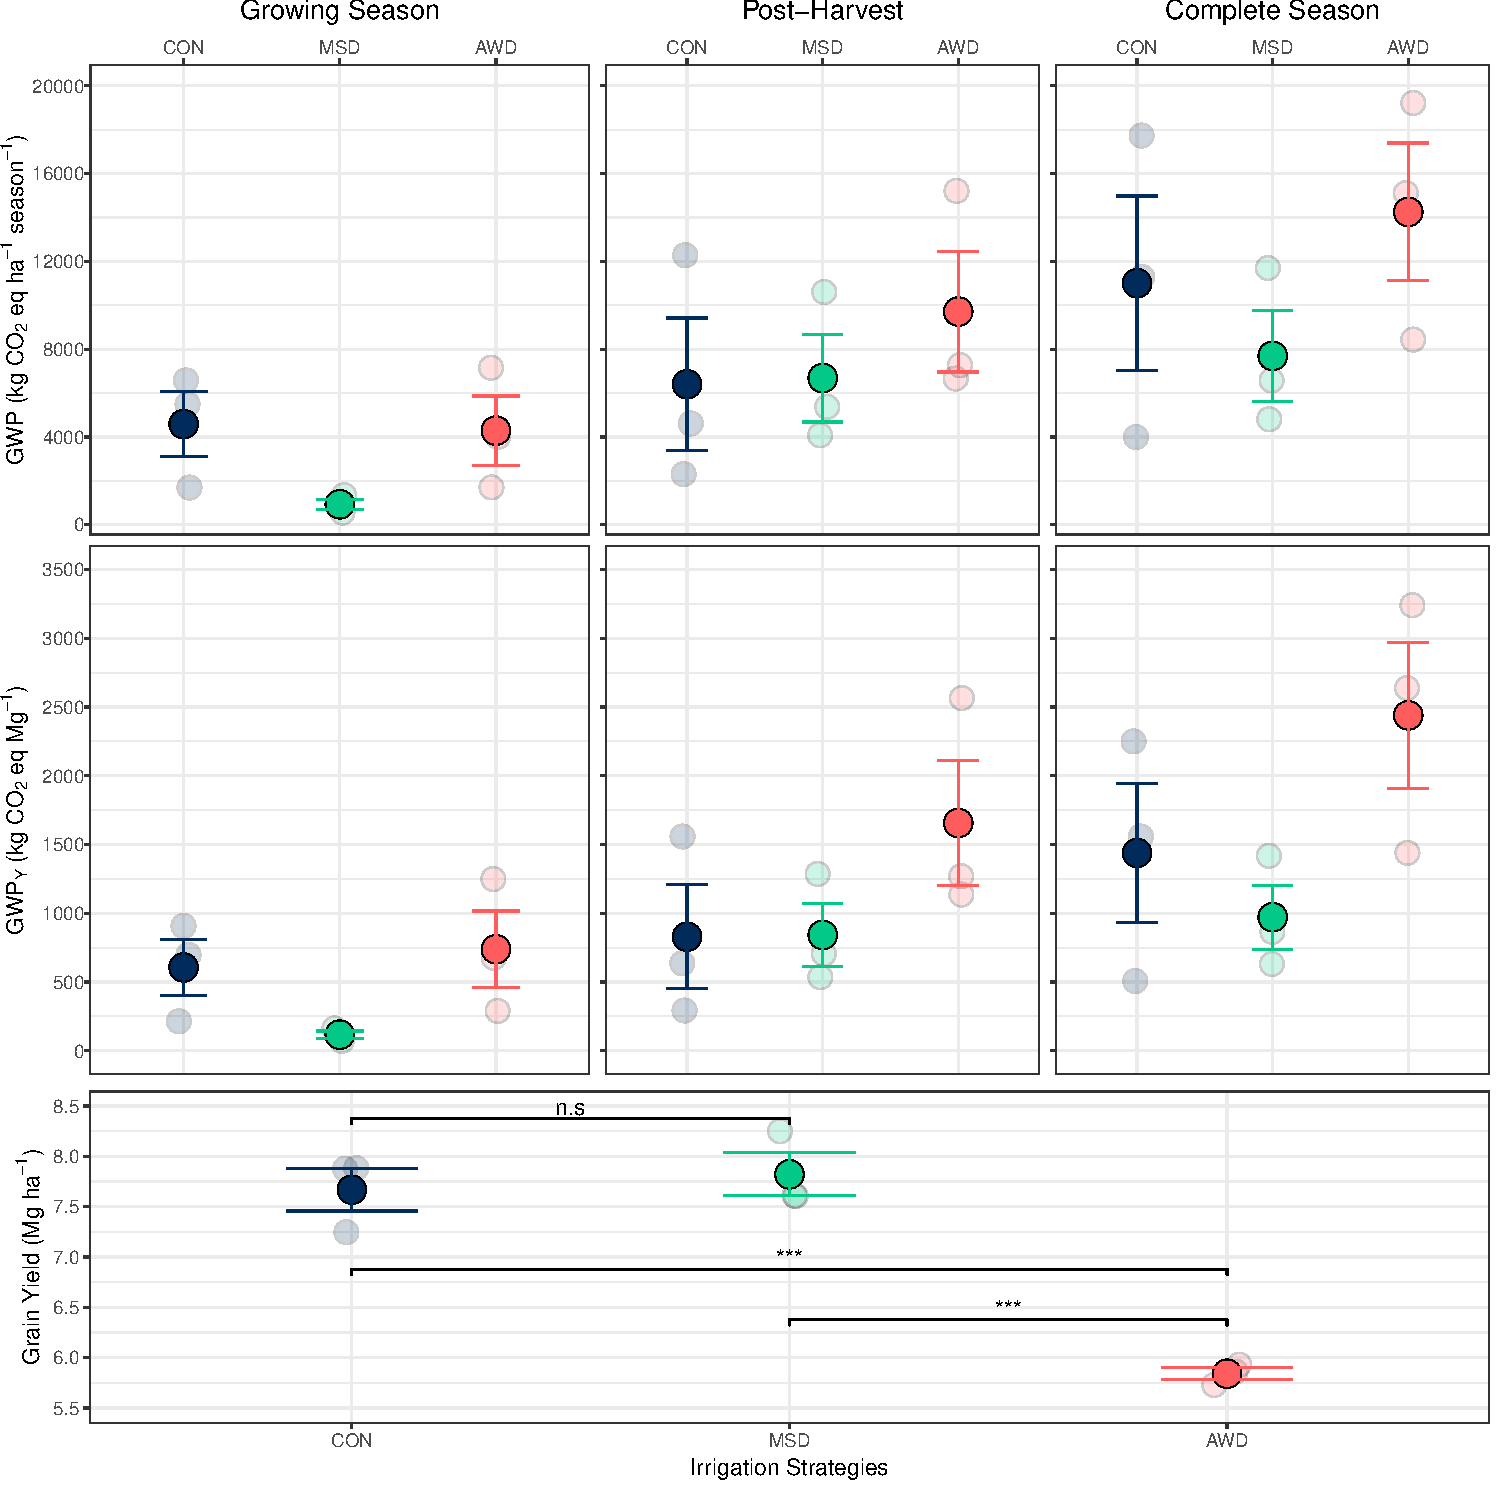
\includegraphics[scale=0.45, center]{Figures/Chapter_2/Yield_GWP_GWPY_arr.pdf}
	\captionof{figure}[GWPY]{Global warming potential (GWP, top plots), yield scaled global warming potential (GWPY, mid plots) and grain yield (bottom plot, in Mg ha$^{-1}$ at 14\% humidity) for the three assessed irrigation strategies. GWP and GWPY are calculated for the rice growing, fallow and complete (both growing and fallow) rice seasons. Solid dots show mean values, transparent dots show values per repetition. Error bars represent standard errors. Significance p-value ($\ast$ $\ast$ $\ast$ \textit{p}$<$0.001, $\ast$ $\ast$ \textit{p}$<$0.01; $\ast$ \textit{p}$<$0.05; n.s.: non significant) indicate statistical differences according to pairwise comparisons between the three assessed irrigation strategies and are only included in Grain Yield (bottom) panel, as no significative differences were found for GWP or GWPY.}  
	\label{GWPY}
\end{figure}
%\vspace{0.5cm}

Once cumulative CH$_{4}$ and N$_{2}$O emissions were accounted for, GWP was calculated and then yield scaled (GWPY) to compare water strategy effects on GHG emissions standardized to CO$_{2}$ equivalents (CO$_{2}$ eq) (Figure \ref{GWPY}). Compared to rice yields from continuously flooded plots (7.7$\pm$0.2 Mg ha$^{-1}$), MSD strategy maintained grain yield levels (7.8$\pm$0.2 Mg ha$^{-1}$) while AWD averaged a 24\% decrease (5.8$\pm$0.1 Mg ha$^{-1}$). This negative effect of AWD management caused an increase in warming potentials when scaling GWP to GWPY for these plots in comparison to other strategies. Overall annual warming potentials (GWP in Mg CO$_{2}$ eq ha$^{-1}$ and GWPY in Mg CO$_{2}$ eq Mg$^{-1}$), considering both growing and fallow seasons, were 11.5$\pm$3.9 and 1.5$\pm$0.5 for continuously flooded plots, 8.0$\pm$2.2 and 1.0$\pm$0.2 for MSD, and 14.6$\pm$3.2 and 2.5$\pm$0.5 for AWD. Even though no significant difference across treatments was identified for GWP ($\chi^2$=1.9, \textit{p}=0.393) or GWPY ($\chi^2$=3.8, \textit{p}=0.148), AWD represented average increases of 26.8\% and 66.2\% in GWP and GWPY, respectively, when compared to continuous flooding. \\ 

\subsection{Microbial biodiversity}

Structure of soil microbial communities varied through the assessed periods (Figure \ref{Beta}). Communities associated to plots managed under AWD strategy were significantly different to those in continuously flooded (growing season: \textit{F}=3.3, \textit{p}=0.001; fallow season: \textit{F}=1.7, \textit{p}=0.014) and in MSD ones (growing season: \textit{F}=2.0, \textit{p}=0.013; fallow season: \textit{F}=1.7, \textit{p}=0.009) through both periods. No significant differences were identified in between continuous flooding and MSD strategies (growing season: \textit{F}=1.5, \textit{p}=0.112; fallow season: \textit{F}=1.0, \textit{p}=0.398).\\

\begin{figure} [ht]
\captionsetup{justification=justified}
	\centering 
	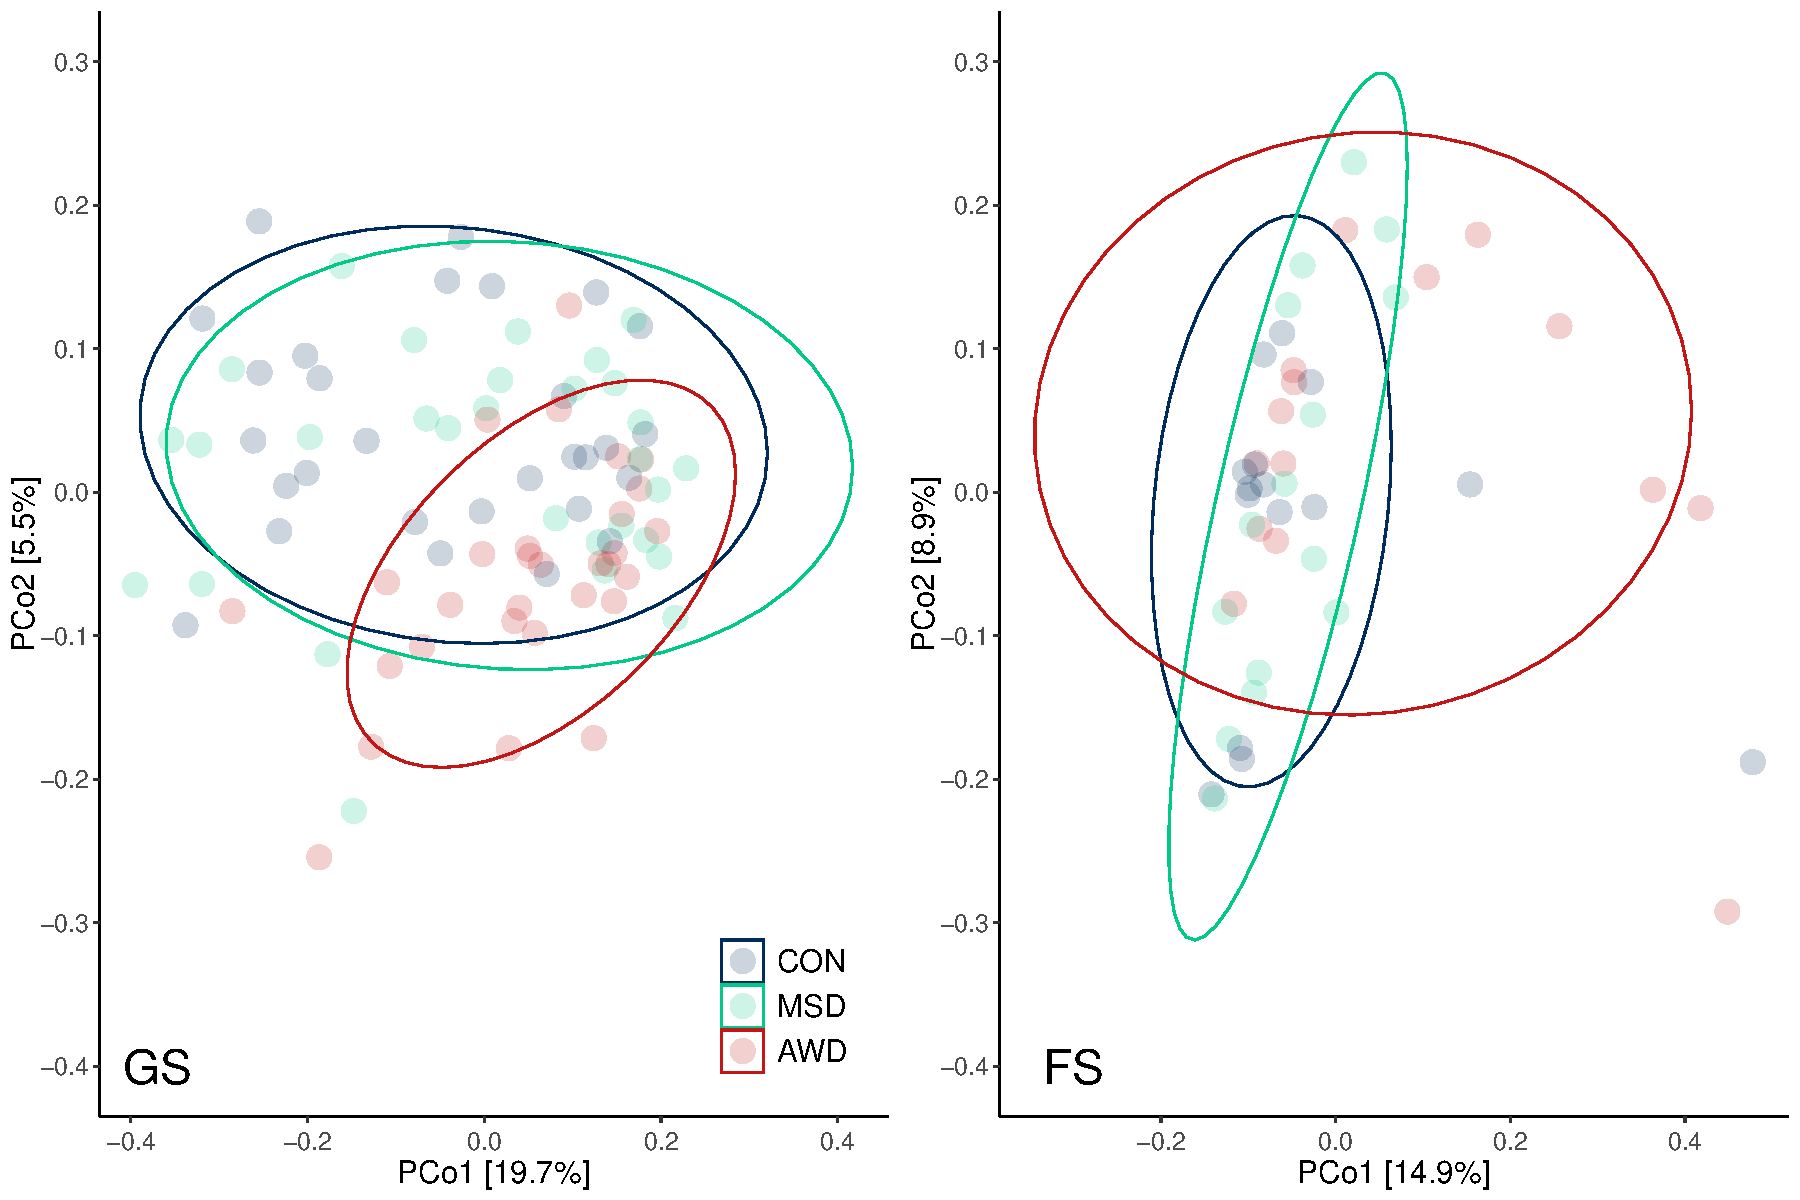
\includegraphics[scale=0.4, center]{Figures/Chapter_2/PCoA_stages_treatGSFS.pdf}
	\captionof{figure}[Beta]{Beta-diversity principal coordinate analysis (PCoA) derived from Bray–Curtis distances of soil microbial communities structure for both assessed periods (GS: Growing season; FS: Fallow season). Communities are clustered in regards to the irrigation strategies corresponding to the plot from which they were sampled.}  	
 \label{Beta}
\end{figure}
%\vspace{0.5cm}

No significant differences were identified among treatments in total bacterial ($\chi^2$=2.4, \textit{p}=0.294) and methanogenic archaeal ($\chi^2$=3.2, \textit{p}=0.205) abundances (Figure \ref{FuncGroups}a.-b.). Overall trends, nevertheless, showed lower total abundances for both groups of organisms in AWD plots when compared to both other irrigation strategies. When accounting for relative abundances among functional groups, populations of both methanogens (\textit{t}=2.9, \textit{p}=0.005) and methanotrophs (\textit{t}=2.3, \textit{p}=0.020) were more abundant in continuously flooded than those in AWD plots. Continuously flooded plots resulted also in higher relative abundance of methanogens than MSD plots (\textit{t}=3.6, \textit{p}=$<$0.001), no significant differences between these strategies was observed for methanotrophs (\textit{t}=1.0, \textit{p}=0.333). No differences in the abundance of alphaproteobacteria methanotrophs were found, whereas relative abundances for gammaproteobacteria methanotrophs within AWD plots resulted significantly lower than those in continuously flooded (\textit{t}=-2.4, \textit{p}=0.019) and MSD (\textit{t}=-2.5, \textit{p}=0.016). \\

\begin{figure} [ht]
\captionsetup{justification=justified}
	\centering 
	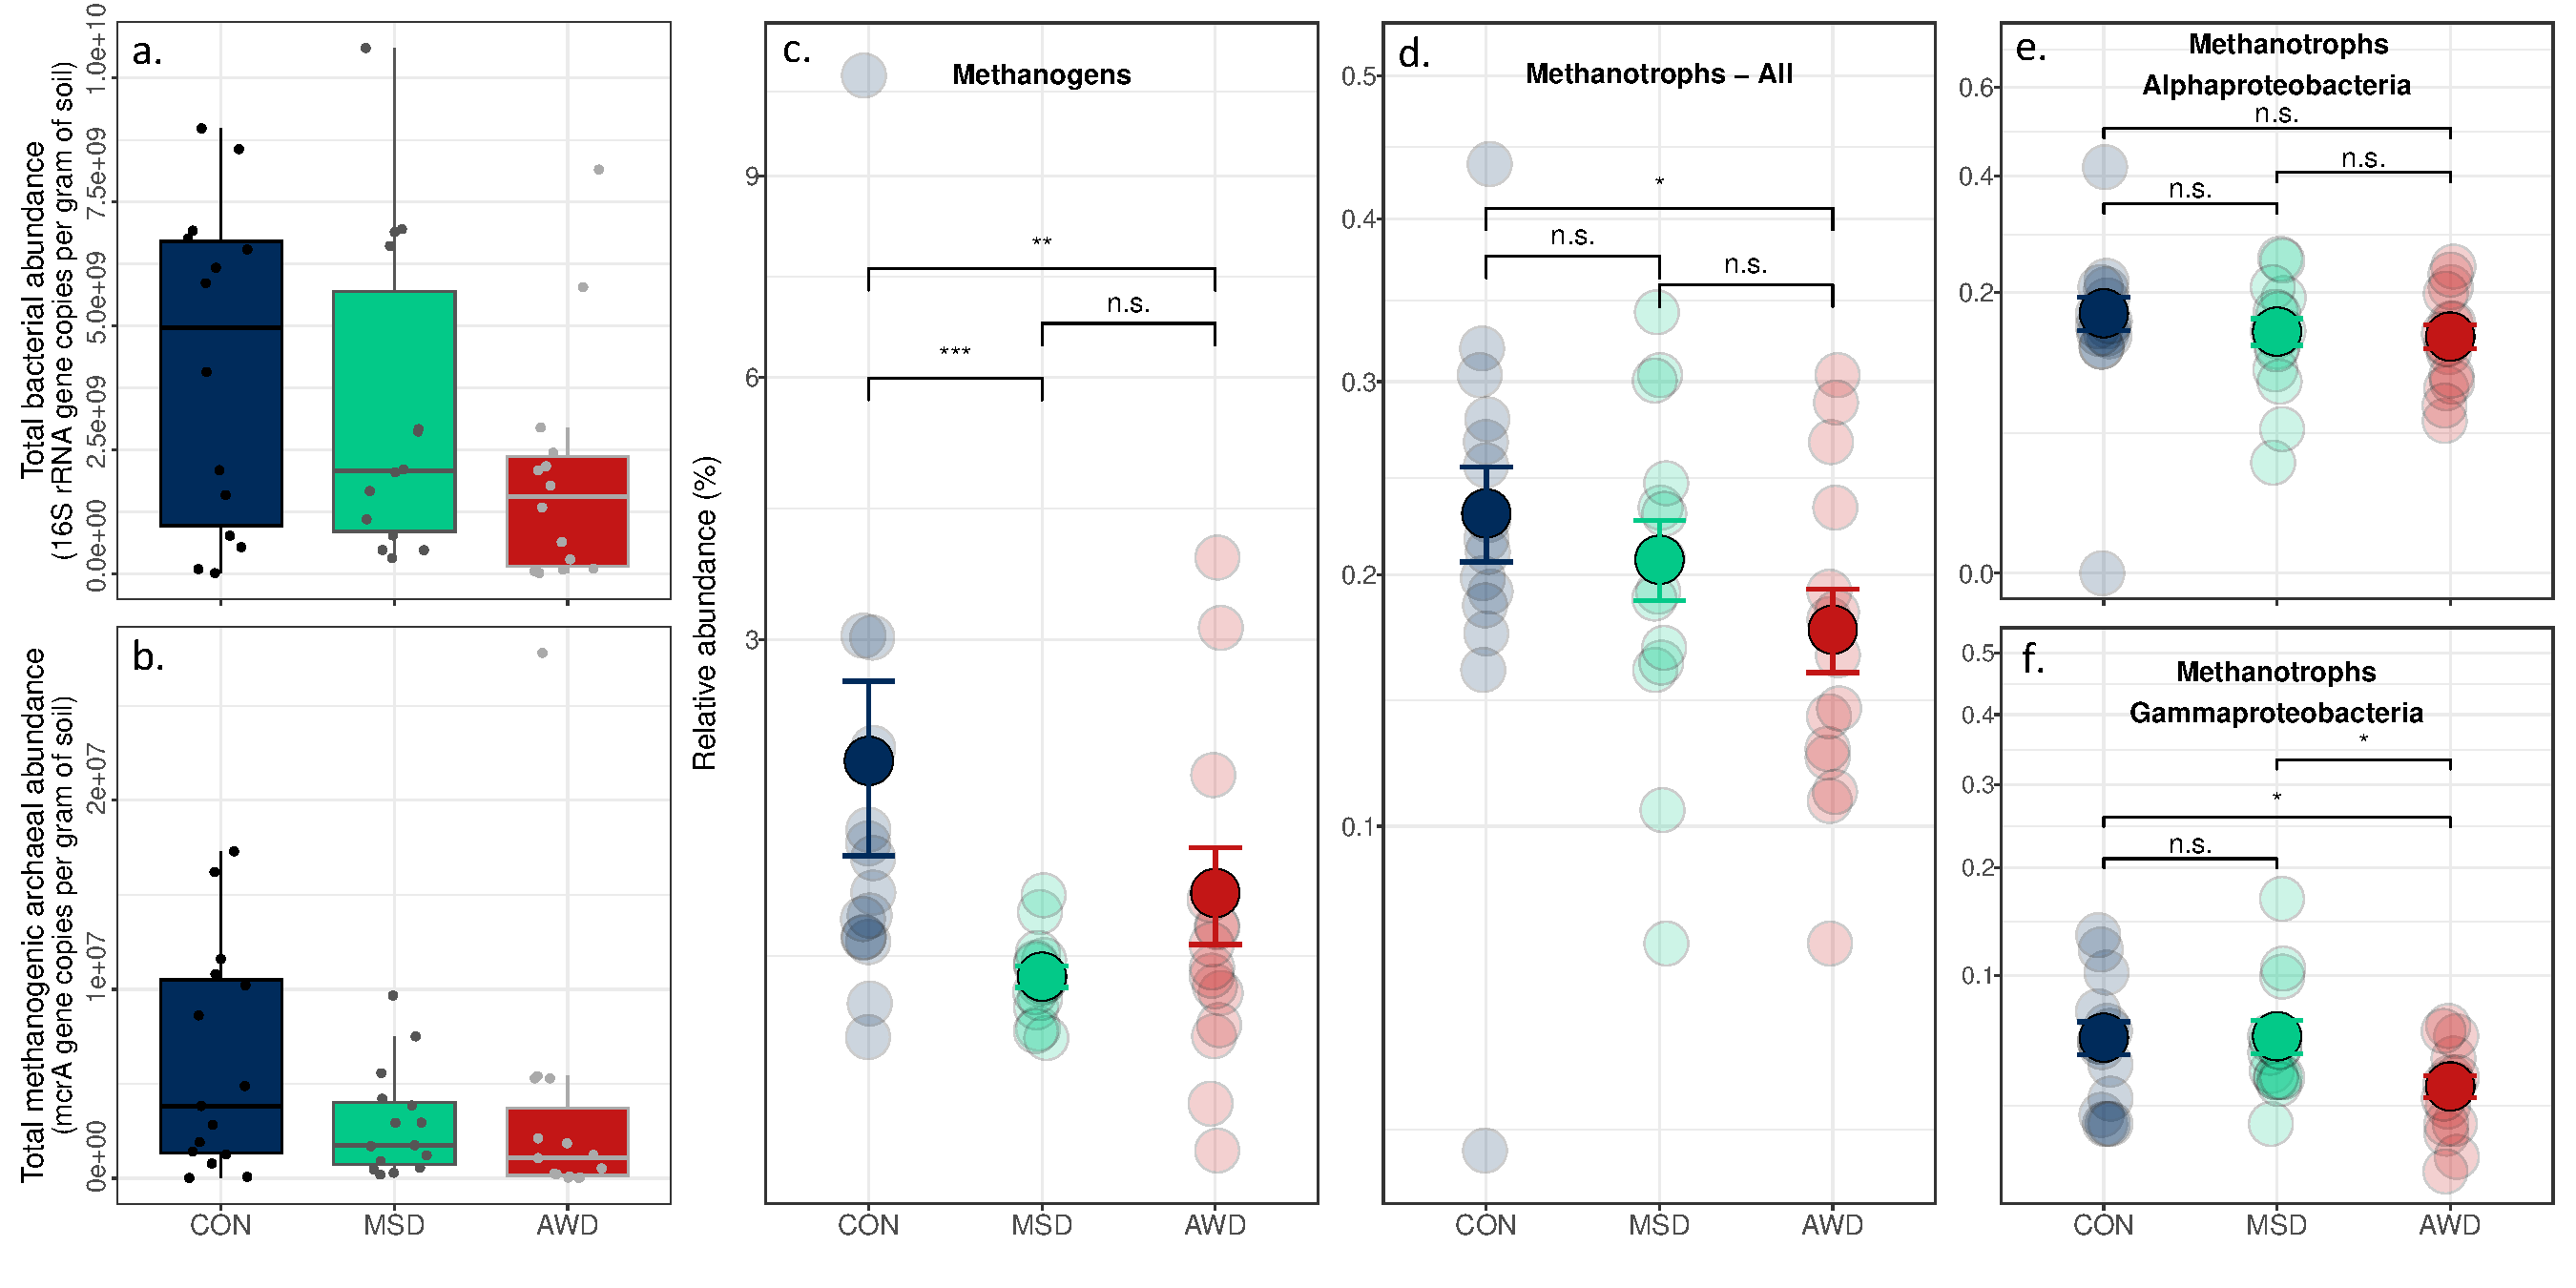
\includegraphics[scale=0.37, center]{Figures/Chapter_2/FuncGroups_plot_arr3_annot.pdf}
	\captionof{figure}[FuncGroups]{Fallow season total and relative abundances of soil microbial communities. Total bacterial (a.) and methanogenic archaeal (b.) abundances according to resulting copies per gram of soil for 16S rRNA and mcrA gene sequences, respectively. Bacterial and archaeal relative abundance (\%) according to their assigned functional groups (Methanogens (c.) and Methanotrophs - All (d.), Alphaproteobacteria (e.) and Gammaproteobacteria (f.)). Significance p-value ($\ast$ $\ast$ $\ast$ \textit{p}$<$0.001, $\ast$ $\ast$ \textit{p}$<$0.01; $\ast$ \textit{p}$<$0.05; n.s.: non significant) indicate statistical differences according to pairwise comparisons between the three assessed irrigation strategies for each functional group model.}  	\label{FuncGroups}
\end{figure}
%\vspace{0.5cm}

\section{Discussion}
\label{sec:discussion}

% Methane emissions 1: FS contribution to overall annual emissions 
Fallow season contribution to total annual cumulative CH$_{4}$ emissions (87\%) surpassed largely that of growing season emissions, as had been previously noted by \cite{martinez2018neglecting} for the Ebro Delta region. Averaged fallow season cumulative CH$_{4}$ emissions within mesocosm units set up from plots kept previously flooded during the growing season (145.7 kg ha$^{-1}$) were comparable to fallow season field measurements recorded at a larger scale for the whole Delta region (163.9 kg ha$^{-1}$, \cite{martinez-eixarch2021a}), peaking as well during October. Higher growing season CH$_{4}$ emissions registered for the region by \cite{martinez-eixarch2021a} (96.6 versus 52.5 kg ha$^{-1}$ recorded in this current study) might have been a product of the high soil clay content in our site, as a strong negative relation between this soil property and CH$_{4}$ emissions was identified in that previous study. Other temperate rice studies resulting in higher emissions in growing than in fallow seasons have either lacked straw incorporation \citep{reba2019} or have being conducted in regions with lower atmospheric temperatures during fallow seasons \citep{fitzgerald2000, adviento-borbe2013, lahue2016, peyron2016, wust-galley2023} (Figure \ref{temp}). Increased microbial activity due to higher fallow season soil temperatures \citep{conrad2023}, and the adaptation of soil microbial communities to such fallow season conditions through several years of rice production under the same edaphoclimatic conditions and agronomic practices \citep{jangid2011, lagomarsino2016a, conrad2020, hester2022}, are potential mechanisms explaining the contrasting CH$_{4}$ emissions pattern in between growing and fallow season in our study system in contrast to other temperate rice agroecosystems. \\ 

% Methane emissions 2: Mitigation during GS and legacy effects over FS
A positive effect of both non-continuous flooding strategies as climate change mitigation practices was observed through a steep decrease in growing season CH$_{4}$ emissions (86\%), when compared to continuously flooded plots. This decrease is higher than the average 53\% CH$_{4}$ emission decrease identified by \cite{jiang2019water} through a global meta-analysis, however, it is in line with that reported by studies in temperate rice systems \citep{linquist2015, lahue2016}. More noteworthy were the effects of these irrigation strategies when observing the following flooded fallow season, where CH$_{4}$ emission patterns changed from AWD being the strategy with lowest to the one with highest emissions. These differences in between CH$_{4}$ emissions during a flooded fallow season from plots previously managed under different irrigation strategies during the growing season suggest the presence of legacy effects of past soil moisture on CH$_{4}$ emissions. \cite{lahue2016} had previously concluded that AWD effects did not extend into fallow seasons under similar management (straw incorporated and flooded fallow season), nevertheless, as discussed above, lower temperatures during fallow seasons might have decreased CH$_{4}$ emissions during that period, hindering potential effects in comparison to our current results. The highest fallow season CH$_{4}$ emissions corresponded to AWD, contradicting the initially hypothesized extended climate change mitigation effect of this strategy over the fallow season. Nonetheless, growing season MSD did manage to maintain lower fallow season CH$_{4}$ emissions when compared to both other strategies. This MSD mitigation effect decreasing CH$_{4}$ emissions through both rice seasons results of great interest as it requires as well significantly less planning and field effort than that of an AWD strategy.\\ 

% Methane emissions 3: cum.CH4, GWP, GWPY, Yield
Although implementing an AWD strategy decreases cumulative CH$_{4}$ emissions during the growing season, when considering its fallow season emission peaks the overall annual effect is negative as cumulative CH$_{4}$ emissions, GWP and GWPY are higher than those registered for both other assessed strategies (Figures \ref{CH4N2O} and \ref{GWPY}). The effects on yields were variable in between non-continuous flooding irrigation strategies as, even though MSD proved to maintain production levels similar to those in continuously flooded plots, a strong decline in grain yield (24\%) was observed for AWD. The main drivers of such decline are the length of drying periods, ground water-table depth and evaporative demand \citep{tuong2003rice}. A significant AWD yield decline of 19\% was previously registered in the same study site by \cite{martinez-eixarch2021}, which identified panicle density and grain number per panicle as the most affected yield components. \cite{monaco2021} found as well that grain number per panicle had significative declines under AWD in comparison to continuous flooding in a similar system. Larger yield reduction in our current study might be explained by a second period of drain-flood cycles during grain ripening, which was not implemented in that previous experience. For the particular agroecosystem assessed in this study, MSD represented a potentially more effective strategy, achieving the lowest cumulative CH$_{4}$ emissions, GWP and GWPY across seasons without grain yield decreases. In contrast to the observed effects on CH$_{4}$ fluxes across both seasons, a lower number of observations (three per irrigation strategy) might have impeded the identification of significant effects of irrigation strategies on cumulative CH$_{4}$ emissions. Further research on these effects is recommended to fully understand the overall impacts of these practices on global change, specifically for rice producing regions with high CH$_{4}$ emissions during fallow seasons.\\ 

% Microbial biodiversity 1: Emission-microbiology transition
The hypothesis of a long-lasting mitigation effect of AWD implemented during the growing season on fallow season CH$_{4}$ emissions derived from the notions of: (i) a decreased grain yield in AWD plots during the previous 2022 season, which was expected to be the case again for the current season, resulting in less biomass produced and less straw incorporated (lower carbon inputs); and (ii) of microbial communities adapting progressively to irrigation practices, reinforcing their effect on GHG emissions over time, as proposed by \cite{lagomarsino2016a}. The rejection of this initial hypothesis required revisiting these assumptions. Lower labile soil organic carbon due to past paddy management, such as lower carbon inputs as a consequence of lower amounts of straw incorporated, can result in decreased CH$_{4}$ emissions \citep{hatala2012}. Nevertheless, even though the prediction of reduced grain yields was met, AWD management did not present lower straw incorporation (Table \ref{straw}). Effects of non-continuous flooding practices over belowground biomass have so far been inconclusive in the literature, as negative \citep{oliver2019} and insignificant \citep{carrijo2018} effects have been reported. No particular differences were observed for root development in between plots in this current study (Table \ref{straw}). No evident differences in carbon input among strategies as an explanatory variable for the registered results suggests that these effects might rather be explained by changes in soil microbial community structure and composition. \\

% Microbial biodiversity 2: Beta diversity and relative abundance
Microbial communities differed among irrigation strategies during the growing season, with AWD showing a particularly different structure than the other strategies (Figure \ref{Beta}). During the subsequent flooded fallow season, microbial communities did not converge into similar structures despite a cease in disturbances (draining events) and plots being subjected to the same flooding conditions. This preserved microbial community divergence across the treatments beyond the implementation of the disturbance reinforces the idea of irrigation strategies legacy effects on CH$_{4}$ emissions. Past soil moisture content effect on microbial community composition and activity has to be considered as an important driver of microbiological processes in soils undergoing flooding and drainage cycles, as previous dry periods are associated with decreased microbial richness and more even communities \citep{banerjee2016}. Structure variation in between irrigation strategies and rice seasons is driven by soil bacterial and archaeal abundance dependency on soil oxic-anoxic conditions, being higher in flooded fields \citep{breidenbach2014}. Accordingly, our results showed lower abundance of methanogenic archaea and methanotrophic bacteria in AWD \citep{hester2022} (Figure \ref{FuncGroups}c.-d.). Legacy effects of drought periods on soil microbial community composition have been also reported in grassland systems \citep{vilonen2023}.\\

% Microbial biodiversity 3: New hypothesis
Soil CH$_{4}$ concentration is one of the controlling factors for methanotrophic growth \citep{jiao2006}. We hypothesize that a high soil CH$_{4}$ availability due to higher methanogenic activity during the growing season might have driven an enrichment of methanotrophic populations under continuous flooding conditions. Intermittent soil aeration in AWD, on the contrary, depleted soil CH$_{4}$ availability during the growing season due to its negative effect on methanogen abundance, leading as well to a decrease in methanotrophic bacteria populations. The relative abundance of gammaproteobacteria was particularly affected by AWD when compared to both other irrigation strategies (Figure \ref{FuncGroups}f.). In contrast to alphaproteobacteria (Figure \ref{FuncGroups}e.), these methanotrophs are able to oxidize CH$_{4}$ also under flooded anoxic conditions \citep{schorn2024}, therefore, a decrease in their abundance within the AWD microbial community can lead to lower methanotrophic activity when moving towards a flooded fallow season. Straw incorporation at the beginning of the fallow season results in large inputs of readily available organic matter and, consecutively, on an increase in CH$_{4}$ production rates by methanogenic archaeal populations \citep{wassmann1993methane}. Since the difference between CH$_{4}$ production and consumption determines resulting emissions \citep{conrad2009global}, a higher consumption by well established methanotrophic bacteria populations in continuously flooded plots may have kept fallow season CH$_{4}$ emissions at lower rates than those in plots where AWD had been implemented. As a result of this, CH$_{4}$ mitigation during the growing season in AWD was eventually offset by the increased fallow CH$_{4}$ emissions. Differences among outcomes from both non-continuous flooding strategies can also be understood through the analysis of their effects on microbial communities. Whereas a unique drainage might have decreased the relative abundance of methanogens surviving into the fallow season when comparing to continuously flooded plots, methanotrophs were apparently more resilient to this single disturbance, as their abundance was unaffected. This contrasting response to drainage periods between methanogens and methanotrophs suggests a divergent ability to recover after drainage events. Alterations in biogeochemical properties of paddy soil driven by changes in soil redox could have also played a role in this differing response. For instance, nutrient cycling (i.e., N and Fe) is modified with alternated reduced and oxic conditions in soils, with further implications in microbial activity \citep{chen2023}. \\

% Microbial biodiversity 4: Activity hypothesis and reach of the study
The current analysis focused on the abundance rather than on the activity of organisms present within soil microbial communities during one rice fallow season. 
Besides growing season soil CH$_{4}$ availability as a driver of fallow season microbial abundances and CH$_{4}$ production and emission, potential change in microbial activity could also be a mechanism involved in these processes.
\cite{breidenbach2014} described how draining fields leads to lower abundances of bacteria and archaea, but also to higher microbial activity (in terms of increased cellular levels of rRNA) as a possible mechanism of stress response of surviving anaerobic microorganisms to be prepared for re-flooding. Methanogenic archaea in AWD plots, even if decreased in numbers compared to continuous flooding ones (Figure \ref{FuncGroups}c.), might have been better prepared to resume their activity once anoxic conditions and carbon input were provided. A steeper depletion of methanogen populations caused by a single and longer drainage in MSD plots could have potentially made this defense mechanism undetectable in comparison to carbon metabolism pathways more prevalent in the overall community, driving the observed fall in CH$_{4}$ emissions for this strategy. Methanotrophs, however, did not seem to follow this same response mechanism as no emission mitigation effect was observed in AWD plots. Drainage and wetting cycles can reduce methane oxidation potential in rice paddy fields \citep{ma2013}. Furthermore, methanotrophic bacteria did not show a strong susceptibility to longer MSD drainage but responded in accordance to the gradient of disturbance in terms of frequency of drainage events. Additionally to growing season soil CH$_{4}$ availability, abundance of methanotrophic microorganisms could be determined as well by the recovery time after each disturbance event, as microbial communities in disturbed soils tend to return to previous stability states with time \citep{jangid2011}. A single disturbance and sufficient time for methanotroph communities to stabilize after it in MSD might explain the observed intermediate effect of this strategy on relative abundance levels. Lower relative abundance of methanogens and populations of methanotrophs large enough to consume their CH$_{4}$ production could explain the positive mitigation effects observed in MSD in terms of cumulative CH$_{4}$, GWP and GWPY. \\

% Discussion closure: Agricultural mgmt and mitigation practice recommendations, and short-term experiment comment
The severe drought conditions under which this experiment was conducted highlight the double role that irrigation strategies might play in rice paddies. Besides their potential mitigation effects due to reduced GHG emissions, they serve as well as climate change adaptation practices allowing farmers to maintain production reducing water use \citep{ye2013}. Our results suggest that a single drain is a more efficient irrigation management addressing GHG emissions in our assessed system, compared to both continuous flooding and AWD. Therefore, considering AWD as a one-size-fits-all solution is not recommended and its scale up should follow proper assessment under local conditions. Specific environmental and agronomic conditions (e.g. high fallow season temperatures) might turn this practice into a detrimental strategy when considering overall annual effects. Even though our study considered the cumulative effect of two years of irrigation strategies, GHG emissions and effects on soil microbial communities correspond to those registered during one growing and its subsequent fallow season, thus representing short-term effects. Further studies considering not only microbial abundance but also their activity through longer time-scale field studies are necessary to determine the exact mechanisms responsible for different effects of irrigation strategies on the presence and prevailing metabolic pathways of specific functional groups of soil microorganisms, and the consequent effects on CH$_{4}$ emissions across rice production seasons.\\ 

\section{Conclusions}
\label{sec:conc}

Under the particular edaphoclimatic conditions and agricultural practices carried out in the Ebro Delta rice agroecosystems, 
% removed after Reviewer #4's suggestions: CH$_{4}$ fluxes peak during the fallow season, dwarfing those observed across the crop growing season. 
a single drainage event, as in MSD irrigation, proved effective as a mitigation strategy considering an overall annual period. Even though AWD is an effective climate change mitigation practice during the growing season, its effects during the fallow season are less clear. Higher CH$_{4}$ emissions during the fallow season suggest potential negative effects of AWD management compared to continuous flooding in terms of overall cumulative CH$_{4}$ emissions, GWP and GWPY. % removed after Reviewer #4's suggestions: Changes in the structure of soil microbial communities can be assessed as an approach to understand the effects of irrigation strategies on CH$_{4}$ emissions across seasons. AWD not only reduced methanogenic archaea, but also methanotrophic bacteria, ultimately leading to an increase in CH$_{4}$ emissions in comparison to continuous flooding. 
The persistence of microbial community structures with reduced abundances of methanogenic archaea and methanotrophic bacteria into the following flooded fallow season can hinder the expected mitigation effect of AWD. Our study suggests a legacy effect of irrigation strategies on soil community structure with implications on the dynamics of GHG emissions in the subsequent season following their implementation. Lower relative abundance of methanogenic archaea and higher presence of methanotrophic organisms under a MSD management might explain its positive potential as a climate change mitigation practice. Implementing an AWD irrigation strategy should not be considered as a one-size-fit-all solution for climate change mitigation in rice agroecosystems. The effects of climate change mitigation practices should be assessed beyond the season in which they are implemented since they may cause persistent effects on GHG emission drivers, such as the composition of soil microbial communities, increasing their potential capacity to alter GHG dynamics.\\

\section*{ACKNOWLEDGEMENTS}
\label{sec:ackn}

This study was funded by the Spanish Ministry of Economy, Trade and Enterprise (MINECO) through the Grant PID2020-118650RR-C31 (funded by MCIN/ AEI/ 10.13039/ 501100011033). The Government of Catalonia funded the predoctoral fellwoship of S.E.-P. through the projects AgriCarboniCat and AgriRegenCat. N.P.-M. is supported by a Spanish ‘Ramón y Cajal’ fellowship (RYC-2021-033599-I). We thank Joan Noguerol for all his support in gas chromotagraphy analysis and Prof. Bruce A. Linquist for his reviews and constructive feedback. We also thank Andrea Bertomeu, Vicent Cebolla, Joan Didac Bertomeu, Raul Llevat, Guillem Rovira and Juan Blas Fernández-Araujo for all their field support. The support of the CERCA Programme, Generalitat de Catalunya, is also acknowledged.

\subsection*{Competing interests statement}
\label{sec:interests}

The authors declare that they have no known competing financial interests or personal relationships that could have appeared to influence the work reported in this paper.

%\pagebreak
 
%\bibliography{cas-refs}

\pagebreak

%\appendix
%\section*{Appendices}
%\label{sec:ann}
%
%\setcounter{figure}{0}
%\renewcommand{\thefigure}{A.\arabic{figure}}

\newcommand{\appendixBtables}{
  \renewcommand{\thetable}{B.\arabic{table}}
  \setcounter{table}{0}
}

\section{Appendix to Chapter 2}
\addcontentsline{toc}{chapter}{Appendix to Chapter 2}
\renewcommand{\thefigure}{B.\arabic{figure}}
\setcounter{figure}{0}
%\renewcommand{\thetable}{B.\arabic{table}}
%\setcounter{table}{0}

\appendixBtables  % ← Ensures tables start with B.1, B.2, etc.

% CH4 Flux with empiric fluxes per plot:

\begin{figure*}[htbp]
\captionsetup{justification=justified}
	\centering 
	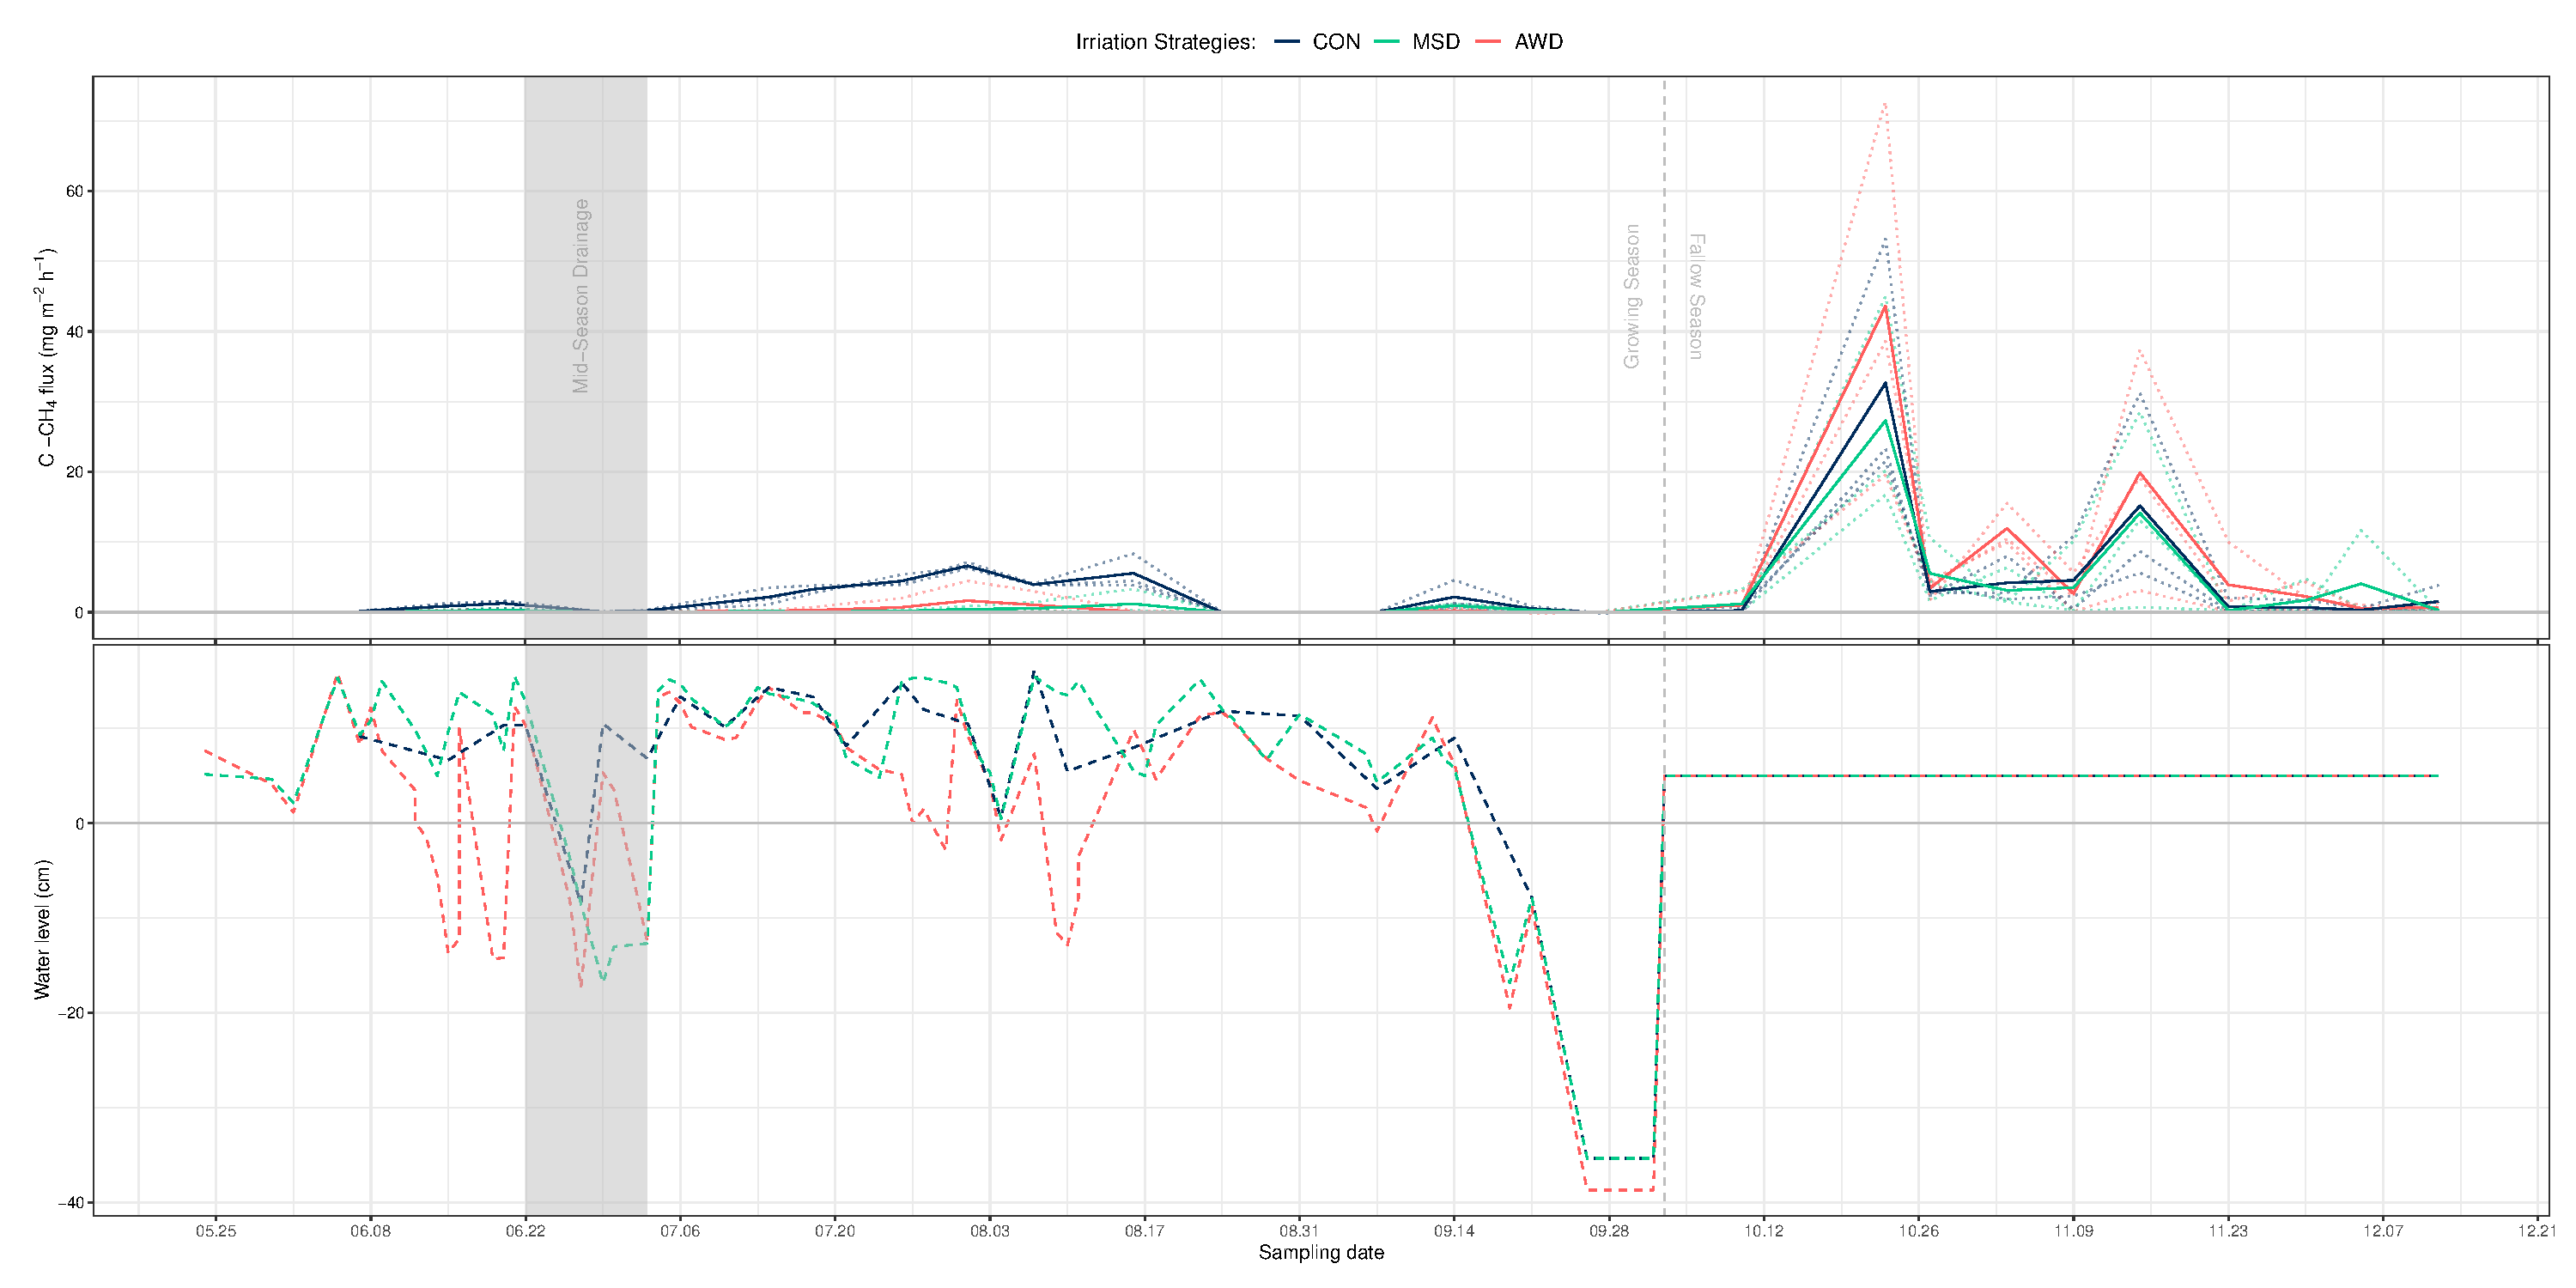
\includegraphics[scale=0.35, center]{Figures/Chapter_2/CH4_flux_water.pdf}
	\captionof{figure}[Treats]{Methane (CH$_{4}$, top panel) emission rates in mg m$^{-2}$ h$^{-1}$, and water level (bottom panel) in cm across the rice growing and fallow seasons for the three assessed irrigation strategies. Discontinuous lines in the top panel are mean emissions per plot, continuous lines are treatment means.}     \label{CH4_plot}
\end{figure*}
%\vspace{0.5cm}\\

% N2O Flux:

\begin{figure*}[htbp]
\captionsetup{justification=justified}
	\centering 
    	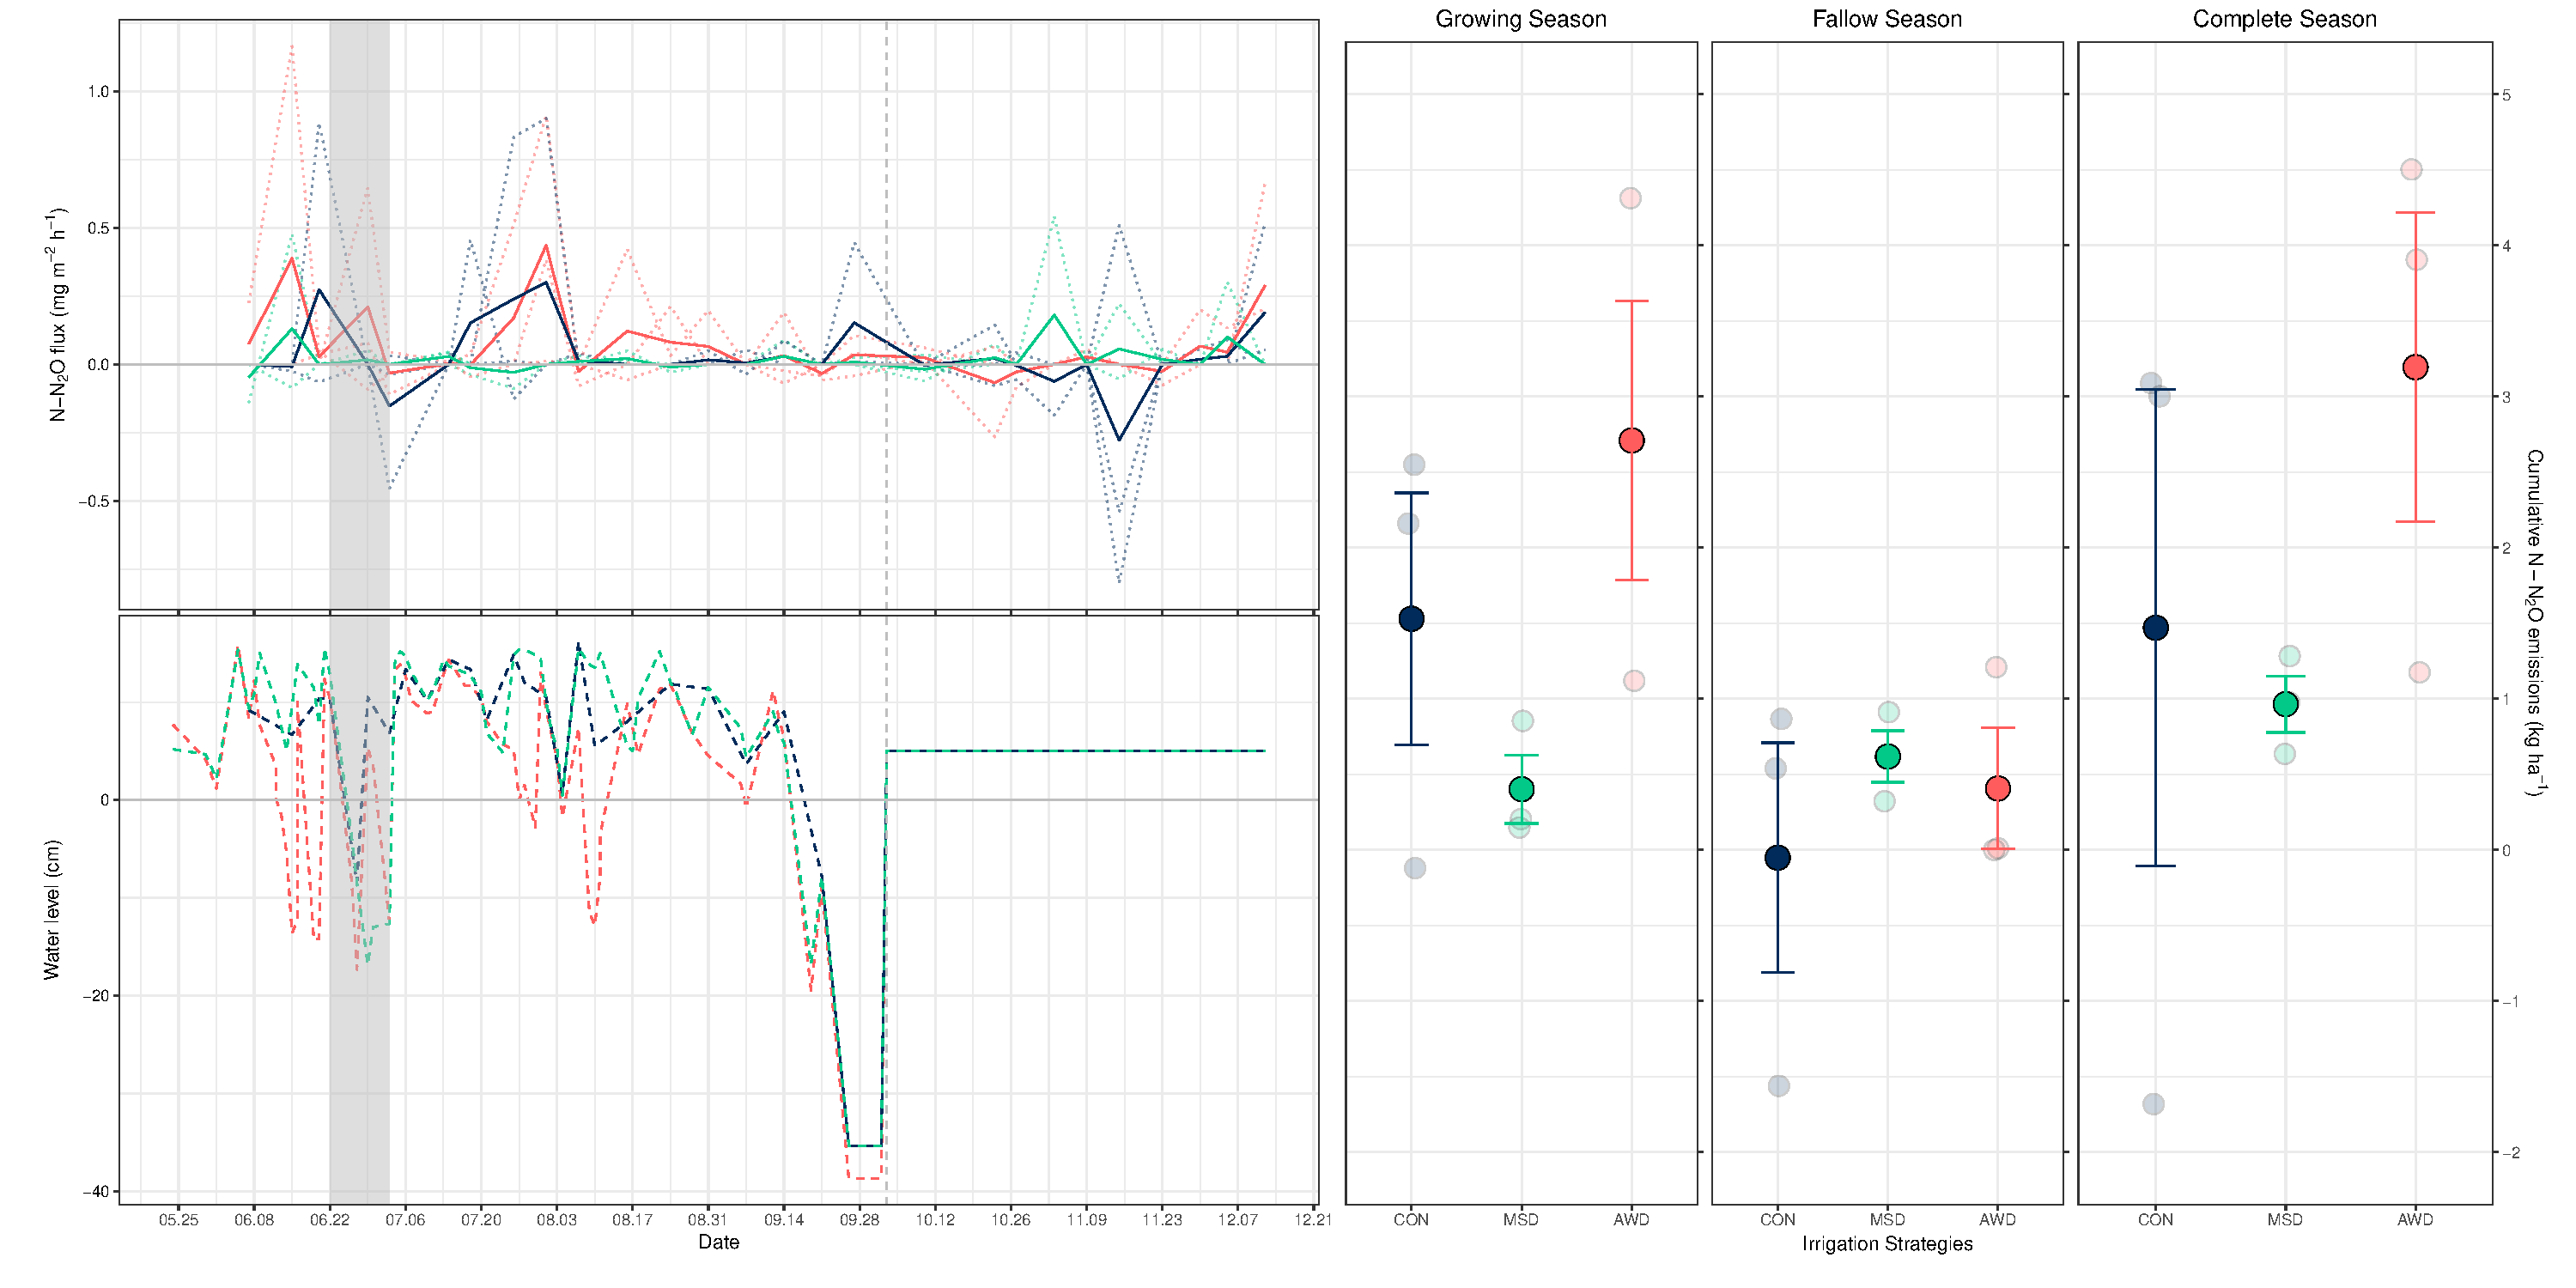
\includegraphics[scale=0.35, center]{Figures/Chapter_2/N2O_flux_acc_water.pdf}
	\captionof{figure}[Treats]{Nitrous oxide (N$_{2}$O, top-left panel) emission rates in mg m$^{-2}$ h$^{-1}$, and water level (bottom-left panel) in cm across the rice growing and fallow seasons for the three assessed irrigation strategies. Discontinuous lines in the top-left panel are mean emissions per plot, continuous lines are treatment means. Right panels show cumulative N$_{2}$O emissions in kg ha$^{-1}$ for the rice growing, fallow and complete (both growing and fallow) rice seasons. Solid dots show mean values, transparent dots show values per repetition. Error bars represent standard errors.}   
	\label{N2O}
\end{figure*}
%\vspace{0.5cm}\\

% Soil properties and Straw incorporated per mesocosm unit:

\begin{table*} [htbp]
    \centering
    \small  
    \begin{tabular}{ c | c | c }
\cline{1-3}
\multicolumn{3}{c}{Soil physicochemical properties} \\
\cline{1-3}
{Parameter} & {Value} & {Unit} \\
\cline{1-3}
{pH} & {8} & {}\\
{Electrical conductivity (25\degree C)} & {0.78} & {dS m$^{-1}$} \\
{Oxidizable organic matter} & {2.83} & {\% d.m.b$^{*}$} \\
{Equivalent Calcium Carbonate} & {36.26} & {\% d.m.b} \\
\cline{1-3}
\multicolumn{3}{c}{Soil nutrients content} \\
\cline{1-3}
{Nutrient} & {Value} & {Unit} \\
\cline{1-3}
{Nitrate} & {7.3} & {mg kg$^{-1}$ d.m.b}\\
{Phosphate} & {19.9} & {mg kg$^{-1}$ d.m.b} \\
{Potassium} & {150} & {mg kg$^{-1}$ d.m.b} \\
{Calcium} & {7,352} & {mg kg$^{-1}$ d.m.b} \\
{Magnesium} & {391} & {mg kg$^{-1}$ d.m.b} \\
{Sodium} & {251} & {mg kg$^{-1}$ d.m.b} \\
\cline{1-3}
\multicolumn{3}{c}{Straw incorporated to mesocosm units} \\
    \cline{1-3}
{Treatment} & {Mean Weight (g)} & {std. error (g)} \\ 
    \cline{1-3} 
CON & 180.00 & 17.54 \\
MSD & 175.04 & 14.69 \\
AWD & 179.22 & 5.16 \\
    \cline{1-3}
\multicolumn{3}{c}{Root biomass per irrigation strategy} \\
    \cline{1-3}
{Treatment} & {Mean Dry Weight (g)} & {std. error (g)} \\ 
    \cline{1-3} 
CON & 1.24 & 0.31 \\
MSD & 1.42 & 0.36 \\
AWD & 1.11 & 0.27 \\
\cline{1-3}
    \end{tabular}
    \caption{Soil description (physicochemical properties and nutrient content), straw incorporated to mesocosm units and root biomass per irrigation strategy. $^{*}$d.m.b = on dry matter basis}
    \label{straw}
\end{table*}

% Mesocosm setup:

\begin{figure} [ht]
\captionsetup{justification=justified}
	\centering 
	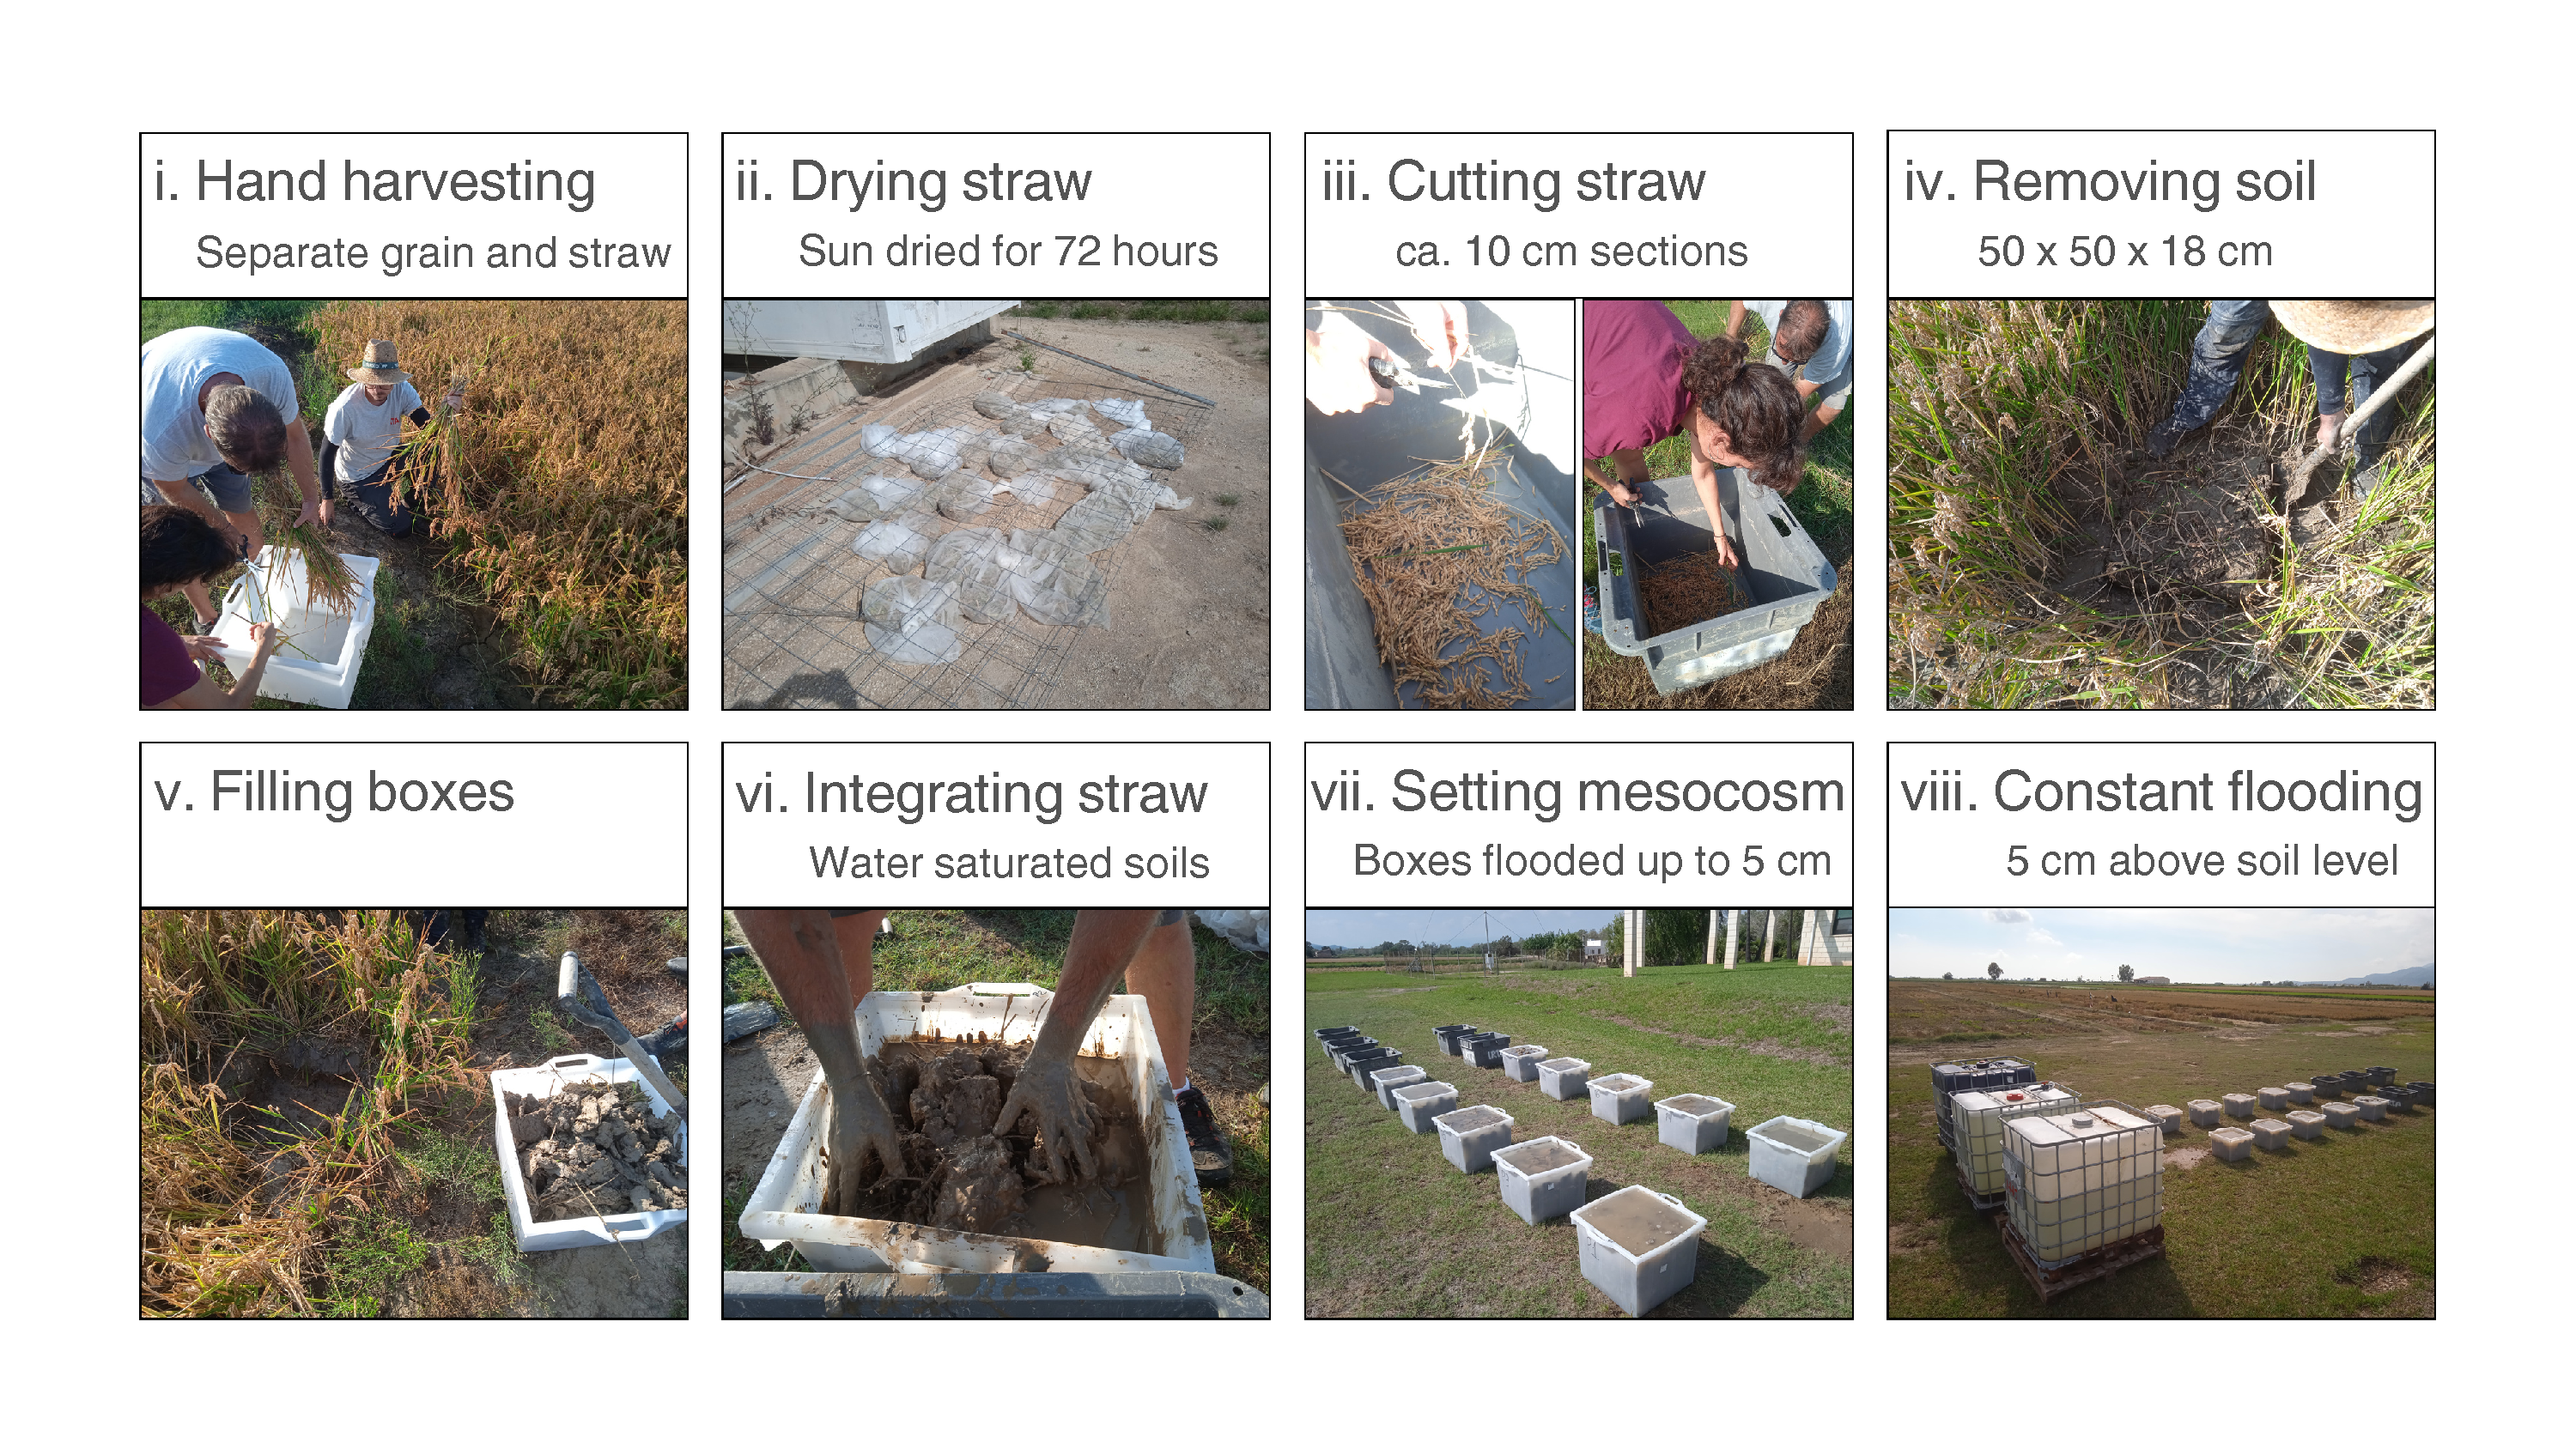
\includegraphics[scale=0.3, center]{Figures/Chapter_2/CERESTRES_meso_2023.pdf}
	\captionof{figure}[lay]{Fallow season mesocosm experiment, setup steps and layout.}  
	\label{meso}
\end{figure}
%\vspace{0.5cm}

% Weather data:

\begin{figure} [ht]
\captionsetup{justification=justified}
	\centering 
	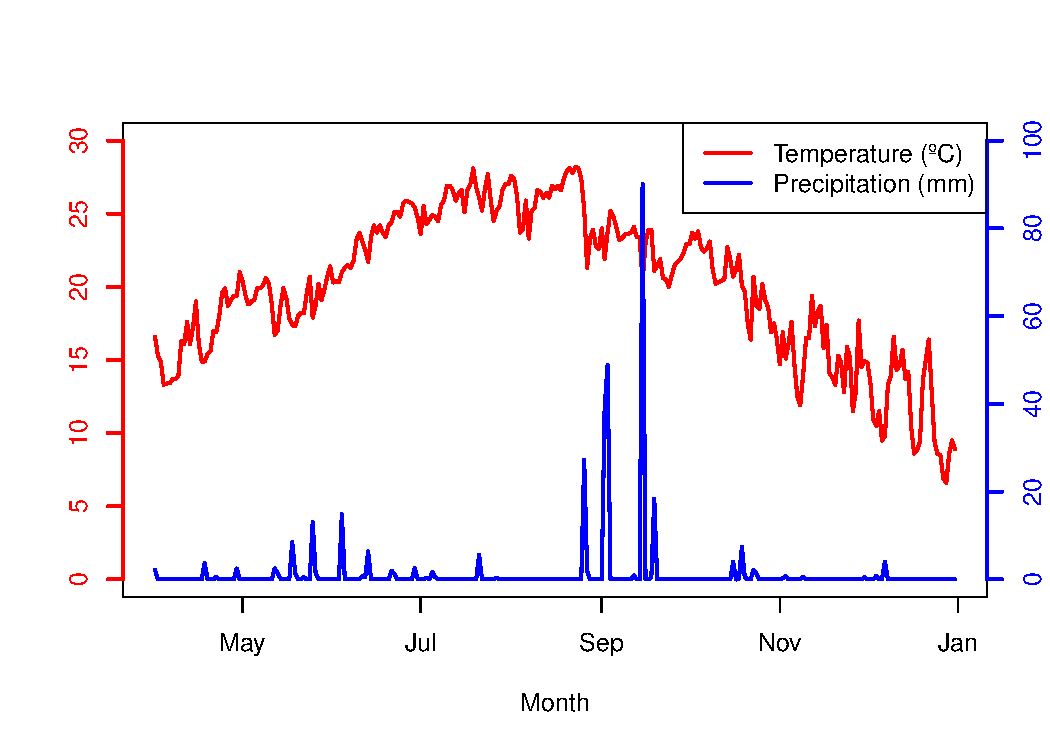
\includegraphics[scale=0.8, center]{Figures/Chapter_2/Meteocat_temp.pdf}
	\captionof{figure}[lay]{Average daily temperature (\degree C) and cumulative daily precipitation (mm) registered by an on-site meteorological station across 2023 growing and fallow seasons.}  
	\label{temp}
\end{figure}
%\vspace{0.5cm}

% Meso vs field physicochemical data:

\begin{figure} [ht]
\captionsetup{justification=justified}
	\centering 
	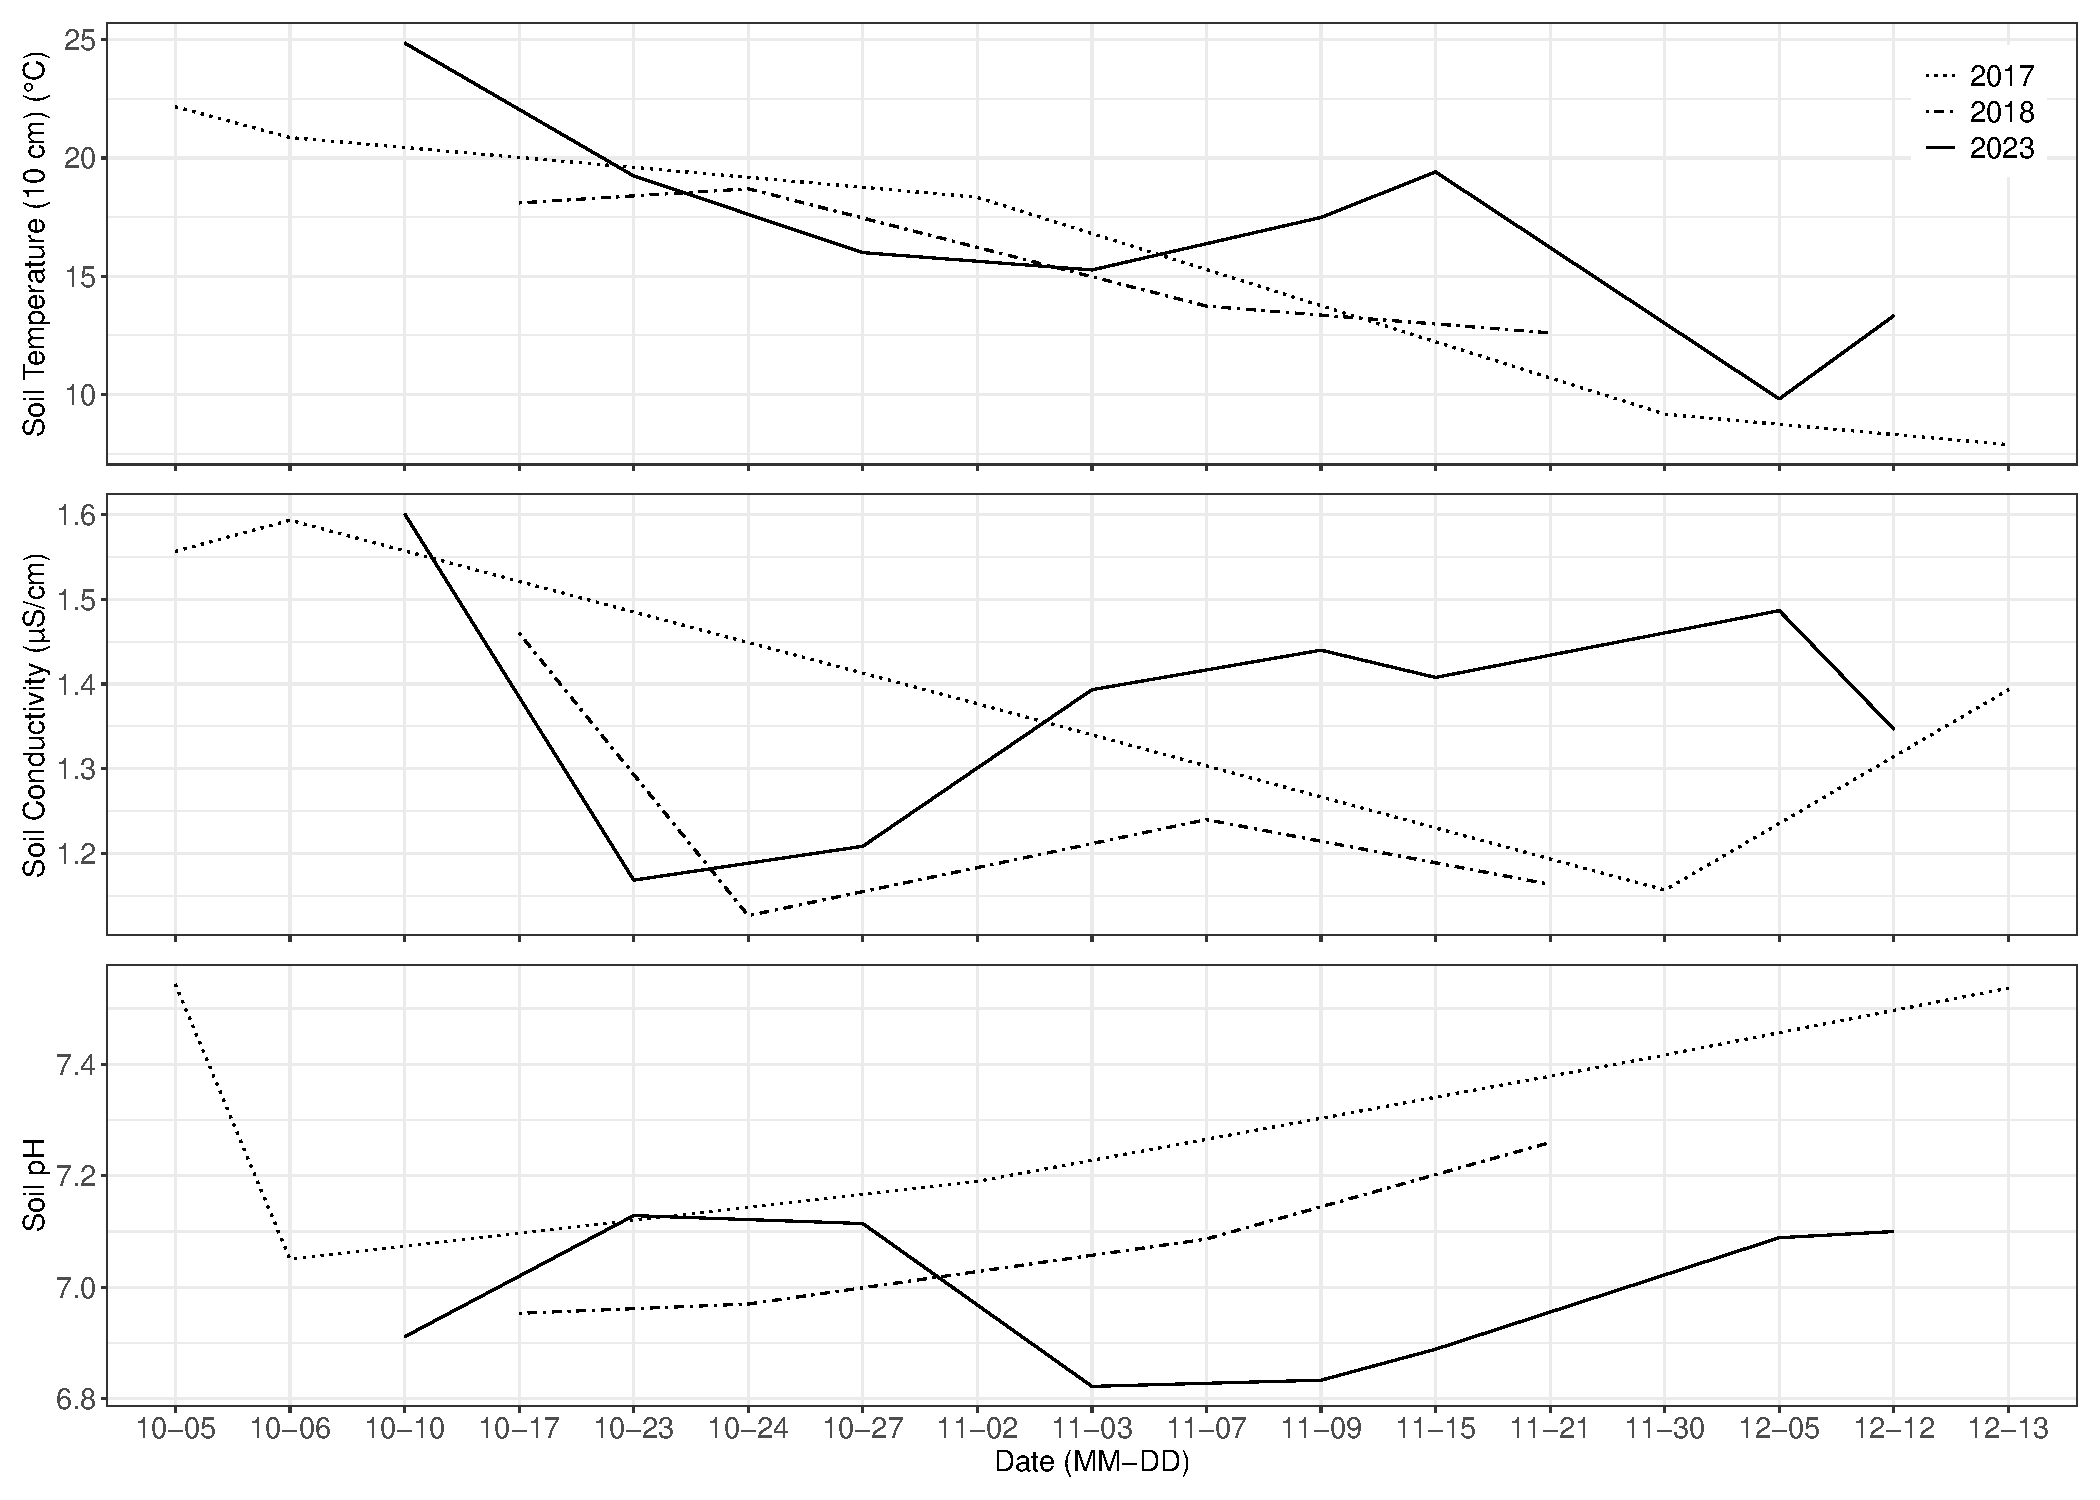
\includegraphics[scale=0.47, center]{Figures/Chapter_2/Meso_vs_Field_Plot.pdf}
	\captionof{figure}[lay]{Soil physicochemical parameters for 2017, 2018 and 2023 flooded fallow seasons. Soil temperature (\degree C) at 10 cm depth, conductivity (µS/cm) and pH. Fallow seasons 2017 and 2018 were assessed in field plots, whereas fallow season 2023 was conducted in mesocosm units. All measurements were done in plots within the IRTA Ebro Experimental Station facilities in Amposta, securing constant soil texture.}  
	\label{meso_field}
\end{figure}
%\vspace{0.5cm}

%\end{document}

% Restore normal figure and table numbering
\renewcommand{\thefigure}{\thechapter.\arabic{figure}}
\setcounter{figure}{0}

\renewcommand{\thetable}{\thechapter.\arabic{table}}
\setcounter{table}{0}
